\documentclass[11pt,a4paper]{article}
\usepackage[utf8]{inputenc}
\usepackage[margin=2.4cm]{geometry}
\usepackage{amsmath,amssymb,amsthm,mathtools}
\usepackage{microtype,booktabs,array,enumitem,float,xcolor}
\usepackage{tikz,pgfplots}
\usetikzlibrary{arrows.meta,positioning,shapes.geometric,calc,fit,backgrounds}
\pgfplotsset{compat=1.16}
\usepackage[most]{tcolorbox}
\usepackage[colorlinks=true,linkcolor=blue!50!black,urlcolor=blue!50!black,citecolor=blue!50!black]{hyperref}

% ---------- numbering: this is lecture 06, sections 6.1 ... ----------
\renewcommand{\thesection}{6.\arabic{section}}
\newcommand{\slr}[1]{\texorpdfstring{\ \emph{(slides #1)}}{ (slides #1)}}
\newcommand{\slrs}[1]{\texorpdfstring{\ \emph{(slide #1)}}{ (slide #1)}}

% ---------- math macros ----------
\newcommand{\R}{\mathbb{R}}
\newcommand{\bx}{\mathbf{x}}
\newcommand{\by}{\mathbf{y}}
\newcommand{\bz}{\mathbf{z}}
\newcommand{\bu}{\mathbf{u}}
\newcommand{\bs}{\mathbf{s}}
\newcommand{\bm}{\mathbf{m}}
\newcommand{\be}{\mathbf{e}}
\newcommand{\bX}{\mathbf{X}}
\newcommand{\bH}{\mathbf{H}}
\newcommand{\bb}{\mathbf{b}}
\newcommand{\bJ}{\mathbf{J}}
\newcommand{\bK}{\mathbf{K}}
\newcommand{\bS}{\mathbf{S}}
\newcommand{\bG}{\mathbf{G}}
\newcommand{\bC}{\mathbf{C}}
\newcommand{\bI}{\mathbf{I}}
\newcommand{\bT}{\mathbf{T}}
\newcommand{\SE}{\mathrm{SE}(3)}
\newcommand{\Sim}{\mathrm{Sim}(3)}
\newcommand{\SL}{\mathrm{SL}(4)}
\newcommand{\N}{\mathcal{N}}
\newcommand{\tr}{\operatorname{tr}}
\DeclareMathOperator*{\argmin}{arg\,min}
\DeclareMathOperator*{\argmax}{arg\,max}
\newcommand{\norm}[2]{\lVert #1\rVert_{#2}}

% ---------- boxes ----------
\tcbset{thmbase/.style={enhanced,breakable,sharp corners=downhill,fonttitle=\bfseries,coltitle=white,
  attach boxed title to top left={yshift=-2mm,xshift=3mm},boxed title style={sharp corners},top=3mm,
  before skip=10pt,after skip=8pt}}
\newtcbtheorem[number within=section]{definition}{Definition}{thmbase,colback=gray!6,colframe=gray!60!black}{def}
\newtcbtheorem[use counter from=definition]{theorem}{Theorem}{thmbase,colback=red!4,colframe=red!55!black}{thm}
\newtcbtheorem[use counter from=definition]{lemma}{Lemma}{thmbase,colback=red!4,colframe=red!55!black}{lem}
\newtcbtheorem[use counter from=definition]{proposition}{Proposition}{thmbase,colback=red!4,colframe=red!55!black}{prop}
\newtcbtheorem[use counter from=definition]{corollary}{Corollary}{thmbase,colback=red!4,colframe=red!55!black}{cor}
\newtcbtheorem[use counter from=definition]{example}{Example}{thmbase,colback=green!4,colframe=green!45!black}{ex}
\newtcbtheorem[use counter from=definition]{algorithm}{Algorithm}{thmbase,colback=violet!4,colframe=violet!60!black}{alg}
\newtcolorbox{intuition}{enhanced,breakable,colback=blue!5!white,colframe=blue!60!black,coltitle=white,
  fonttitle=\bfseries,title=Intuition,left=2mm,right=2mm,boxrule=0.6pt,before skip=6pt,after skip=10pt}

% ---------- placeholder for photos that must be copied from the slides ----------
\newcommand{\imgph}[3][4.5cm]{%
\begin{figure}[htbp]\centering
\begin{tikzpicture}
\draw[dashed,gray,thick] (0,0) rectangle (0.88\linewidth,#1);
\node[align=center,gray] at (0.44\linewidth,0.5*#1) {\textbf{[ insert image here ]}\\ take it from \textbf{slide #2}};
\end{tikzpicture}
\caption{#3}
\end{figure}}

% ---------- tikz styles ----------
\tikzset{>={Stealth[length=2mm]},
 var/.style={circle,draw,thick,minimum size=7.5mm,inner sep=1pt},
 fac/.style={rectangle,draw,fill=black,minimum size=2.4mm,inner sep=0pt},
 blk/.style={rectangle,draw,rounded corners=2pt,thick,align=center,font=\small,inner sep=4pt},
 star5/.style={star,star points=5,draw,inner sep=1.5pt,minimum size=4mm}}
\pgfmathdeclarefunction{gauss}{3}{\pgfmathparse{1/(sqrt(2*pi*#3))*exp(-((#1-#2)^2)/(2*#3))}}

\title{\textbf{Foundations of Spatial AI}\\[2pt] Lecture 06 --- Simultaneous Localization and Mapping\\[4pt]\large Detailed lecture notes}
\author{Notes on the slides of L.~Di Giammarino and E.~Giacomini\\ Sapienza University of Rome, October 12, 2026}
\date{}

\begin{document}
\maketitle
\tableofcontents

\section*{About these notes}
The notes follow the slide deck in order; every \verb|\section| and \verb|\subsection| carries the title of the corresponding slide(s) and its slide range. Formulas on the slides are embedded as pictures, so the formal content (definitions, lemmas, theorems, proofs) was reconstructed from the references quoted in the slide footers (Thrun--Burgard--Fox, Stachniss, Dellaert--Kaess, Mur-Artal et al., Lovegrove et al.\ and others) and from lectures 01 and 05 (Lie groups, bundle adjustment). Dashed empty boxes mark photographs or screenshots that must be copied from the indicated slide; all other figures are redrawn in TikZ/pgfplots.

\textbf{Notation.} World-to-camera poses $\bT_i\in\SE$ (as in lecture 05); 3D points $\bX_j$ (or $\mathbf x_j^w$); pixel observations $\mathbf u_{ij}$; $\pi(\cdot)$ is the pinhole projection including intrinsics; $\norm{\mathbf v}{\Omega}^2=\mathbf v^\top\Omega\,\mathbf v$ is the squared Mahalanobis norm. The letter $\bH$ is the Gauss--Newton matrix of Section~6.3, while the EKF measurement Jacobian is called $\bC_t$.

\section*{Agenda and Learning Objectives \slr{1--2}}
\textbf{Agenda:} 6.1 The SLAM problem; 6.2 Filtering; 6.3 Graph-based SLAM; 6.4 The visual SLAM pipeline; 6.5 Research directions.

After the lecture you should be able to:
\begin{enumerate}[nosep]
\item formulate SLAM as joint estimation of trajectory and map, and derive the Kalman filter and EKF-SLAM together with their cost;
\item formulate graph-based SLAM as least squares over a factor graph, solve it with Gauss--Newton, and relate its sparsity to marginalization;
\item describe the threads of a keyframe-based visual SLAM system: tracking, local mapping, loop detection and loop correction.
\end{enumerate}

% =====================================================================
\section{The SLAM Problem \slr{3--6}}
\subsection{The SLAM Problem \slrs{3}}

\begin{definition}{SLAM}{slam}
\emph{Simultaneous localization and mapping} computes, at the same time, the camera poses (the trajectory) $\bx_{1:t}=\{\bx_1,\dots,\bx_t\}$ and the map of the environment $\bm$, given the measurements $\bz_{1:t}$ (and, if available, controls $\bu_{1:t}$), i.e.\ the posterior
\[
p(\bx_{1:t},\bm\mid \bz_{1:t},\bu_{1:t}).
\]
\emph{Localization} estimates the poses given the map; \emph{mapping} builds the map given the poses.
\end{definition}

SLAM is a \emph{chicken-or-egg problem}: a map is needed to localize, and a pose estimate is needed to build a map. Without any map, chaining relative motion estimates (\emph{dead reckoning}) accumulates error without bound.

\begin{proposition}{Dead-reckoning drift}{drift}
If each relative motion estimate carries independent zero-mean error of variance $\sigma^2$ per axis, the position variance after $t$ steps is $t\sigma^2$, so the standard deviation grows as $\sigma\sqrt t$ and is unbounded.
\end{proposition}
\begin{proof}
The estimated position is $\sum_{k=1}^t(\Delta_k+\varepsilon_k)$ with independent $\varepsilon_k$; variances of independent terms add. \qedhere
\end{proof}
\begin{intuition}
With $\sigma=1$\,cm per step, after $1000$ steps the $1\sigma$ error is $\sqrt{1000}\approx 32$\,cm, even though no single step was bad. Orientation errors are worse: a small heading error bends the whole subsequent path. A map that is \emph{re-observed} gives absolute references and stops this growth.
\end{intuition}

\begin{figure}[htbp]\centering
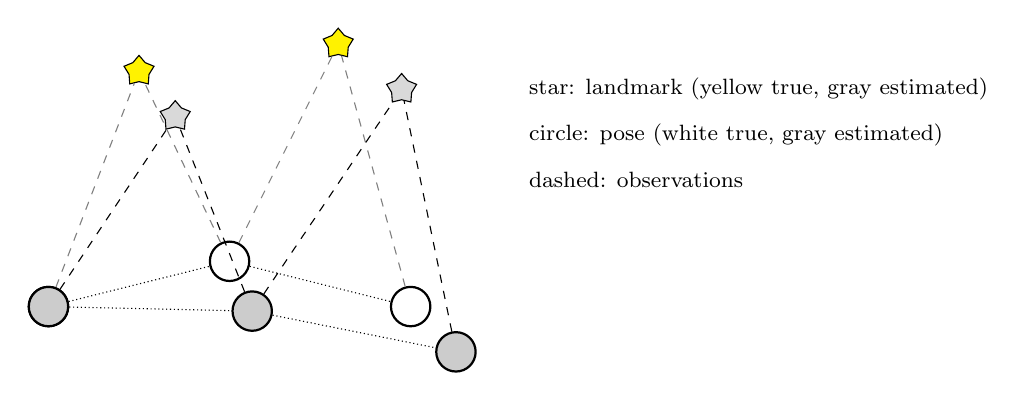
\begin{tikzpicture}[scale=1.15]
\def\tp{(0,0),(2,0.5),(4,0)}
% true poses
\node[var,minimum size=5mm] (t0) at (0,0) {};
\node[var,minimum size=5mm] (t1) at (2,0.5) {};
\node[var,minimum size=5mm] (t2) at (4,0) {};
% estimated poses
\node[var,minimum size=5mm,fill=gray!40] (e0) at (0,0) {};
\node[var,minimum size=5mm,fill=gray!40] (e1) at (2.25,-0.05) {};
\node[var,minimum size=5mm,fill=gray!40] (e2) at (4.5,-0.5) {};
% landmarks
\node[star5,fill=yellow] (L1) at (1,2.6) {};
\node[star5,fill=yellow] (L2) at (3.2,2.9) {};
\node[star5,fill=gray!30] (l1) at (1.4,2.1) {};
\node[star5,fill=gray!30] (l2) at (3.9,2.4) {};
\draw[densely dotted] (t0)--(t1)--(t2);
\draw[densely dotted] (e0)--(e1)--(e2);
\foreach \a/\b in {t0/L1,t1/L1,t1/L2,t2/L2} \draw[dashed,gray] (\a)--(\b);
\foreach \a/\b in {e0/l1,e1/l1,e1/l2,e2/l2} \draw[dashed] (\a)--(\b);
\node[font=\footnotesize,anchor=west] at (5.2,2.4) {star: landmark (yellow true, gray estimated)};
\node[font=\footnotesize,anchor=west] at (5.2,1.9) {circle: pose (white true, gray estimated)};
\node[font=\footnotesize,anchor=west] at (5.2,1.4) {dashed: observations};
\end{tikzpicture}
\caption{Redrawn from slide 3: true and estimated poses/landmarks and the observations linking them. Estimated poses drift away from the truth while the landmarks keep them mutually consistent.}
\end{figure}

\subsection{Cameras for SLAM \slrs{4}}
Cameras are compact, accurate, non-invasive, well understood, and today cheap and ubiquitous. Images carry \emph{appearance}: two rooms that look identical to a 2D laser scanner can be told apart by a camera. Applications range from augmented reality and vision-based navigation to self-driving cars, mobile devices, inspection drones and VR headsets. The cost: a camera senses geometry only indirectly, through photometric effects, and a single camera measures \emph{no depth}.

\begin{proposition}{Scale ambiguity of a monocular camera}{scale}
Let a scene $\{\bX_j\}$ and camera poses $\{(\mathbf R_i,\mathbf t_i)\}$ produce pixels $\mathbf u_{ij}=\pi(\mathbf R_i\bX_j+\mathbf t_i)$. For any $s>0$, the scene $\{s\bX_j\}$ with translations $\{s\mathbf t_i\}$ produces exactly the same pixels.
\end{proposition}
\begin{proof}
$\mathbf R_i(s\bX_j)+s\mathbf t_i=s(\mathbf R_i\bX_j+\mathbf t_i)$, and the perspective projection satisfies $\pi(s\mathbf p)=\pi(\mathbf p)$ because it divides by the depth. \qedhere
\end{proof}
\begin{intuition}
A photograph of a toy house and of a real house can be identical. A single camera therefore recovers the world only \emph{up to a similarity} (rotation, translation \emph{and} scale: 7 degrees of freedom), which is why monocular maps also drift in scale (Section~6.4).
\end{intuition}

\imgph[4.2cm]{4}{Maps built from one camera: sparse features of a room (left) and a dense desktop (right).}

\subsection{SLAM and Structure-from-Motion \slrs{5}}
The unknowns and the error are those of lecture 05: camera poses $\bT_i$ (world to camera), 3D points $\bX_j$, and the reprojection error of every observation. Both problems stem from the same maximum a posteriori formulation; the \emph{setting} differs.

\begin{center}\small
\begin{tabular}{p{5.6cm}p{6.6cm}}
\toprule
\textbf{Structure-from-motion (lecture 05)} & \textbf{SLAM}\\\midrule
Unordered set of images, all available from the start & Frames arrive one at a time; solved incrementally as measurements arrive\\
Solved offline, analyzing all images at once & Pose and map needed at every frame, in real time\\
No notion of returning to a place & Returning to a visited place closes a loop and corrects long-term drift\\\bottomrule
\end{tabular}
\end{center}
\begin{intuition}
SfM is like developing all holiday photos and then assembling the 3D model at home; SLAM is like navigating a city while drawing the map as you walk. Same maths, very different time budget.
\end{intuition}

\subsection{Running Example: VBR Campus \slrs{6}}
\textbf{VBR} (Vision Benchmark in Rome) was recorded hand-held and by car with a global-shutter stereo camera of wide baseline, a 3D LiDAR, an IMU and an RTK-GPS. Its ground truth refines the RTK-GPS with LiDAR bundle adjustment, accurate to $\pm 3$\,cm over 1.5\,km; its six datasets cover over 40\,km. The running example of the lecture is a sequence of around 11\,km.

\imgph[5cm]{6}{VBR: sensor-rig reference frames (camera left/right CL, CR, LiDAR $L$, IMU $I$) and two point-cloud/map renderings of the Rome sequences.}

% =====================================================================
\section{Filtering: From the Bayes Filter to EKF-SLAM \slr{7--13}}
\subsection{SLAM as a Graphical Model \slrs{8}}
The camera poses and the map are unknown; the measurements are observed. Without odometry, as with a single camera, a motion model alone links consecutive poses.

\begin{definition}{Full and online SLAM}{fullonline}
\emph{Full SLAM} estimates the whole trajectory and the map, $p(\bx_{1:t},\bm\mid\bz_{1:t},\bu_{1:t})$. \emph{Online SLAM} keeps only the current pose,
\[
p(\bx_t,\bm\mid\bz_{1:t},\bu_{1:t})=\int\!\!\cdots\!\!\int p(\bx_{1:t},\bm\mid\bz_{1:t},\bu_{1:t})\,d\bx_1\cdots d\bx_{t-1},
\]
i.e.\ it \emph{marginalizes} the past poses, and the integrals are solved recursively one step at a time.
\end{definition}

\begin{figure}[htbp]\centering
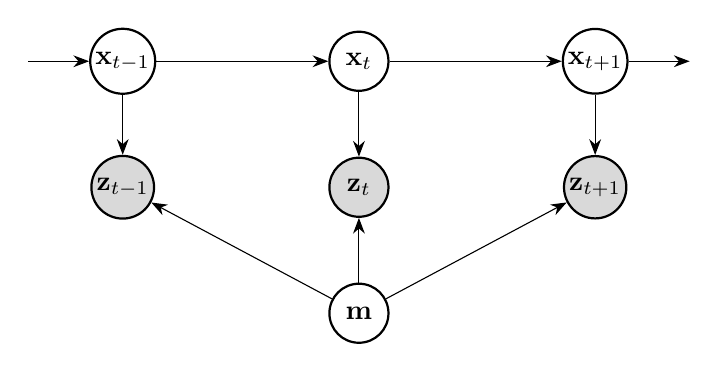
\begin{tikzpicture}
\foreach \i/\x/\l in {0/0/{t-1},1/3/{t},2/6/{t+1}}{
 \node[var] (x\i) at (\x,0) {$\bx_{\l}$};
 \node[var,fill=gray!30] (z\i) at (\x,-1.6) {$\bz_{\l}$};
}
\node[var] (m) at (3,-3.2) {$\bm$};
\draw[->] (x0)--(x1); \draw[->] (x1)--(x2);
\draw[->] (-1.2,0)--(x0); \draw[->] (x2)--(7.2,0);
\foreach \i in {0,1,2}{ \draw[->] (x\i)--(z\i); \draw[->] (m)--(z\i);}
\end{tikzpicture}
\caption{Graphical model of SLAM (slide 8): poses form a Markov chain, the map is static, and each (gray, observed) measurement depends on the current pose and the map. Controls are omitted, as in the monocular case.}
\end{figure}
\begin{intuition}
Full SLAM keeps the entire path (a growing problem, solved later by graphs); online SLAM forgets the past path but remembers what it taught us, packed inside a single Gaussian over the current pose and the map. Marginalizing is ``summing over everything I no longer care about''.
\end{intuition}

\subsection{The Bayes Filter \slrs{9}}
Let $\bs_t=(\bx_t,\bm)$ be the state: camera pose and map.

\begin{theorem}{Recursive Bayes filter}{bayes}
Let $\mathrm{bel}(\bs_t)=p(\bs_t\mid\bz_{1:t},\bu_{1:t})$. Under the Markov assumptions, one frame at a time:
\begin{align*}
\overline{\mathrm{bel}}(\bs_t)&=\int p(\bs_t\mid\bs_{t-1},\bu_t)\,\mathrm{bel}(\bs_{t-1})\,d\bs_{t-1} &&\text{(prediction)}\\
\mathrm{bel}(\bs_t)&=\eta\; p(\bz_t\mid\bs_t)\,\overline{\mathrm{bel}}(\bs_t)&&\text{(update)}
\end{align*}
where $p(\bs_t\mid\bs_{t-1},\bu_t)$ is the \emph{motion model}, $p(\bz_t\mid\bs_t)$ the \emph{measurement model} and $\eta$ a normalizer.
\end{theorem}
\begin{proof}
By Bayes' rule, $\mathrm{bel}(\bs_t)=\eta\,p(\bz_t\mid\bs_t,\bz_{1:t-1},\bu_{1:t})\,p(\bs_t\mid\bz_{1:t-1},\bu_{1:t})$. Given the state, the current measurement is independent of the past, so the first factor is $p(\bz_t\mid\bs_t)$. For the second factor, the law of total probability gives $\int p(\bs_t\mid\bs_{t-1},\bz_{1:t-1},\bu_{1:t})\,p(\bs_{t-1}\mid\bz_{1:t-1},\bu_{1:t})\,d\bs_{t-1}$; the state is Markov, so $p(\bs_t\mid\bs_{t-1},\dots)=p(\bs_t\mid\bs_{t-1},\bu_t)$, and $\bu_t$ carries no information on $\bs_{t-1}$, so the last factor is $\mathrm{bel}(\bs_{t-1})$. \qedhere
\end{proof}
\begin{intuition}
Two beats, forever: \emph{predict} (move the belief with the motion model, which \emph{widens} it, since motion adds uncertainty) and \emph{update} (multiply by how well each hypothesis explains the new image, which \emph{narrows} it). The one-dimensional example below follows slide 9: a camera on a line.
\end{intuition}

\begin{example}{Camera on a line}{line}
Prior $\N(0,1)$. Motion model: move $+1$ with noise variance $1$, so the prediction is $\N(1,\,1+1)=\N(1,2)$. Measurement $z=2$ with noise variance $1$. The posterior is the normalized product of the prediction and the measurement likelihood: $\sigma^2=(2^{-1}+1^{-1})^{-1}=2/3$ and $\mu=\tfrac{2}{3}\big(\tfrac{1}{2}\cdot 1+\tfrac{1}{1}\cdot 2\big)=5/3$.
\end{example}
\begin{figure}[htbp]\centering
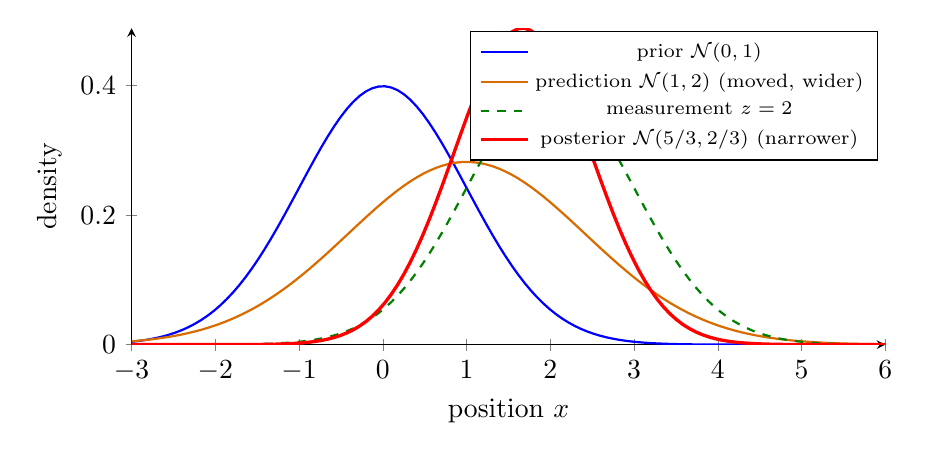
\begin{tikzpicture}
\begin{axis}[width=0.92\linewidth,height=5.6cm,xlabel={position $x$},ylabel={density},ymin=0,xmin=-3,xmax=6,domain=-3:6,samples=120,no markers,axis lines=left,legend style={font=\scriptsize,at={(0.99,0.99)},anchor=north east}]
\addplot[blue,thick]{1/sqrt(2*pi)*exp(-((x)^2)/2)}; \addlegendentry{prior $\N(0,1)$}
\addplot[orange!85!black,thick]{1/sqrt(4*pi)*exp(-((x-1)^2)/4)}; \addlegendentry{prediction $\N(1,2)$ (moved, wider)}
\addplot[green!50!black,thick,dashed]{1/sqrt(2*pi)*exp(-((x-2)^2)/2)}; \addlegendentry{measurement $z=2$}
\addplot[red,very thick]{1/sqrt((4/3)*pi)*exp(-((x-1.6667)^2)/(4/3))}; \addlegendentry{posterior $\N(5/3,2/3)$ (narrower)}
\end{axis}
\end{tikzpicture}
\caption{The Bayes filter in one dimension (slide 9): prediction shifts and widens the belief, the measurement narrows it.}
\end{figure}

\subsection{Kalman Filter and Extended Kalman Filter \slrs{10}}
With Gaussian noise the belief stays Gaussian, $\mathrm{bel}(\bs_t)=\N(\boldsymbol\mu_t,\Sigma_t)$. Let the models be $\bs_t=g(\bs_{t-1},\bu_t)+\boldsymbol\varepsilon_t$, $\boldsymbol\varepsilon_t\sim\N(0,\mathbf R_t)$ and $\bz_t=h(\bs_t)+\boldsymbol\delta_t$, $\boldsymbol\delta_t\sim\N(0,\mathbf Q_t)$. The \emph{extended Kalman filter} (EKF) linearizes both around the current estimate, with Jacobians $\bG_t=\partial g/\partial\bs\,|_{\boldsymbol\mu_{t-1}}$ and $\bC_t=\partial h/\partial\bs\,|_{\bar{\boldsymbol\mu}_t}$.

\begin{algorithm}{Extended Kalman filter step}{ekf}
\textbf{Predict:} $\bar{\boldsymbol\mu}_t=g(\boldsymbol\mu_{t-1},\bu_t)$, \quad $\bar\Sigma_t=\bG_t\Sigma_{t-1}\bG_t^\top+\mathbf R_t$.\\[3pt]
\textbf{Update:} $\bS_t=\bC_t\bar\Sigma_t\bC_t^\top+\mathbf Q_t$ (innovation covariance), \quad $\bK_t=\bar\Sigma_t\bC_t^\top\bS_t^{-1}$ (Kalman gain),\\
$\boldsymbol\mu_t=\bar{\boldsymbol\mu}_t+\bK_t\big(\bz_t-h(\bar{\boldsymbol\mu}_t)\big)$, \quad $\Sigma_t=(\bI-\bK_t\bC_t)\bar\Sigma_t$.
\end{algorithm}

\begin{theorem}{Kalman filter (linear case)}{kf}
If $g(\bs,\bu)=\mathbf A\bs+\mathbf B\bu$ and $h(\bs)=\mathbf C\bs$, the Jacobians are $\bG_t=\mathbf A$ and $\bC_t=\mathbf C$, and the EKF equations give the \emph{exact} posterior. This is Kalman's recursive filter for discrete-time linear systems.
\end{theorem}
\begin{proof}
The prediction is a linear map of a Gaussian plus Gaussian noise, hence Gaussian with the stated mean and covariance. For the update, $(\bs_t,\bz_t)$ is jointly Gaussian with $\mathrm{cov}(\bz_t)=\mathbf C\bar\Sigma\mathbf C^\top+\mathbf Q=\bS$ and $\mathrm{cov}(\bs_t,\bz_t)=\bar\Sigma\mathbf C^\top$. Conditioning a joint Gaussian gives $\mathbb E[\bs\mid\bz]=\bar{\boldsymbol\mu}+\bar\Sigma\mathbf C^\top\bS^{-1}(\bz-\mathbf C\bar{\boldsymbol\mu})$ and $\mathrm{cov}=\bar\Sigma-\bar\Sigma\mathbf C^\top\bS^{-1}\mathbf C\bar\Sigma=(\bI-\bK\mathbf C)\bar\Sigma$. \qedhere
\end{proof}
\begin{intuition}
The gain $\bK$ is a trust dial between model and sensor. In 1D with $\bar\sigma^2=2$ and measurement noise $q=1$: $K=\bar\sigma^2/(\bar\sigma^2+q)=2/3$, so the posterior mean moves two thirds of the way from the prediction ($1$) toward the measurement ($2$), giving $5/3$, exactly Example~\ref{ex:line}; the variance shrinks to $(1-K)\bar\sigma^2=2/3$. For nonlinear $g,h$ the EKF is only an approximation: it converges in the linear case but can \emph{diverge} if nonlinearities are large, because Jacobians are evaluated once, at the current estimate.
\end{intuition}

\subsection{The EKF-SLAM State \slrs{11}}
EKF-SLAM estimates the camera and the positions of all the points with \emph{one} Gaussian: a single mean and a single joint covariance,
\[
\boldsymbol\mu=\begin{pmatrix}\bx_c\\\by_1\\\vdots\\\by_N\end{pmatrix},\qquad
\Sigma=\begin{pmatrix}\Sigma_{cc}&\Sigma_{cm}\\\Sigma_{mc}&\Sigma_{mm}\end{pmatrix}.
\]
In MonoSLAM the camera block $\bx_c$ has 13 numbers (position 3, orientation quaternion 4, linear velocity 3, angular velocity 3); each point adds 3, so the state has $13+3N$ entries and $\Sigma$ has $(13+3N)^2$. The off-diagonal blocks are the \emph{correlations} between the camera and the points and between the points. The filter cycle is: state prediction (the motion model moves the camera block only), measurement prediction, measurement, data association, update (all blocks change). The camera starts at the origin of its own frame; a new point enters the state when first observed.

\newcommand{\covmat}[3]{%
\begin{tikzpicture}[scale=0.85]
\foreach \i/\xa/\xb in {0/0/1.4,1/1.4/2.1,2/2.1/2.8,3/2.8/3.5}{
 \foreach \j/\ya/\yb in {0/0/1.4,1/1.4/2.1,2/2.1/2.8,3/2.8/3.5}{
  \ifnum\i=0 \ifnum\j=0 \def\c{#1}\else\def\c{#2}\fi\else \ifnum\j=0 \def\c{#2}\else\def\c{#3}\fi\fi
  \fill[\c] (\xa,-\ya) rectangle (\xb,-\yb);
 }}
\foreach \p in {0,1.4,2.1,2.8,3.5}{\draw[gray] (\p,0)--(\p,-3.5); \draw[gray] (0,-\p)--(3.5,-\p);}
\node[font=\scriptsize] at (0.7,0.3) {$\bx_c$}; \node[font=\scriptsize] at (1.75,0.3) {$\by_1$};
\node[font=\scriptsize] at (2.45,0.3) {$\cdots$}; \node[font=\scriptsize] at (3.15,0.3) {$\by_N$};
\end{tikzpicture}}
\begin{figure}[htbp]\centering
\covmat{red!55}{red!30}{gray!20}\qquad\qquad\covmat{red!55}{red!40}{red!30}
\caption{Which blocks of the EKF-SLAM covariance change (red). Left, prediction: only the camera block and its correlations, $\Sigma_{mm}$ is untouched. Right, update: every block changes.}
\end{figure}

\begin{proposition}{Cost of EKF-SLAM}{ekfcost}
The prediction touches only $\Sigma_{cc}$ and $\Sigma_{cm}$ (the Jacobian of $g$ is $\mathrm{diag}(\bG_c,\bI)$), but the update has a dense gain $\bK$, so it modifies the \emph{whole} covariance: $O(N^2)$ time per step and $O(N^2)$ memory for $N$ points.
\end{proposition}
\begin{proof}
Since $g$ moves only the camera, $\bG_t=\mathrm{diag}(\bG_c,\bI)$, giving $\bar\Sigma_{cc}=\bG_c\Sigma_{cc}\bG_c^\top+\mathbf R$, $\bar\Sigma_{cm}=\bG_c\Sigma_{cm}$ and $\bar\Sigma_{mm}=\Sigma_{mm}$. In the update, $\Sigma\leftarrow\Sigma-\bK\bS\bK^\top$ with $\bK=\bar\Sigma\bC^\top\bS^{-1}$; because all points are correlated with the camera, $\bK$ has no zero blocks and the rank-update is dense. \qedhere
\end{proof}
\begin{intuition}
Numbers: with $N=100$ points the state has $313$ entries and $\Sigma$ about $98{,}000$ numbers: trivial. With $N=10{,}000$ points, $30{,}013^2\approx 9\times10^8$ entries, about $7.2$\,GB in double precision, \emph{and} touched at every frame. Correlations are a feature (observing one point improves the others) but they are what makes the filter expensive.
\end{intuition}

\subsection{Example: MonoSLAM \slrs{12}}
\textbf{MonoSLAM} is EKF-SLAM with a single camera: it recovers the 3D trajectory of a camera moving rapidly through an unknown scene, at 30\,Hz on a standard PC, and drives live augmented reality from a hand-held camera.
\begin{itemize}[nosep]
\item \textbf{Motion model:} constant linear and angular velocity, with unknown accelerations as Gaussian noise; a hand-held camera has no control input. With $\bx_c=(\mathbf r,\mathbf q,\mathbf v,\boldsymbol\omega)$: $\mathbf r\leftarrow\mathbf r+(\mathbf v+\mathbf V)\Delta t$, $\mathbf q\leftarrow\mathbf q\otimes\mathbf q\big((\boldsymbol\omega+\boldsymbol\Omega)\Delta t\big)$, $\mathbf v\leftarrow\mathbf v+\mathbf V$, $\boldsymbol\omega\leftarrow\boldsymbol\omega+\boldsymbol\Omega$, with $\mathbf V,\boldsymbol\Omega$ Gaussian impulses.
\item \textbf{Measurement model:} pinhole projection of each point, with radial distortion.
\item \textbf{Active search:} the innovation covariance $\bS$ defines an ellipse around each predicted feature, and only these ellipses are searched, for at most 10 or 12 features per frame.
\item About 100 features at 30\,Hz take 19\,ms of the 33\,ms of a frame.
\end{itemize}
\begin{figure}[htbp]\centering
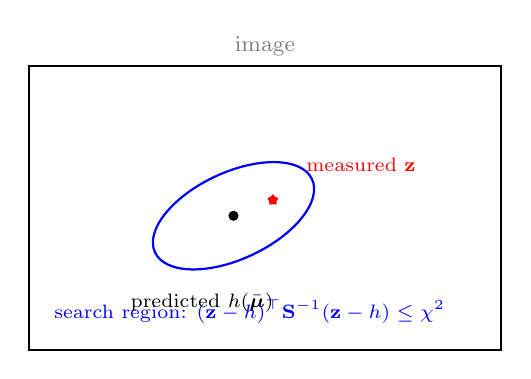
\begin{tikzpicture}
\draw[thick] (0,0) rectangle (6,3.6);
\node[font=\footnotesize,gray] at (3,3.85) {image};
\node[fill=black,circle,inner sep=1.3pt,] (p) at (2.6,1.7) {};
\node[font=\scriptsize,anchor=north] at (2.2,0.85) {predicted $h(\bar{\boldsymbol\mu})$};
\draw[thick,blue,rotate around={25:(2.6,1.7)}] (2.6,1.7) ellipse (1.1 and 0.55);
\node[fill=red,star,star points=5,inner sep=1pt] at (3.1,1.9) {};
\node[font=\scriptsize,anchor=west,red] at (3.4,2.35) {measured $\bz$};
\node[font=\scriptsize,blue,anchor=north west] at (0.2,0.75) {search region: $(\bz-h)^\top\bS^{-1}(\bz-h)\le\chi^2$};
\end{tikzpicture}
\caption{Active search (slide 12): the EKF predicts where a feature should appear and how uncertain that prediction is; only the ellipse is searched.}
\end{figure}
\begin{intuition}
Instead of scanning the whole image for each of 100 features, the filter says ``it must be about \emph{here}, give or take this much''. Searching a few small ellipses is why a 1990s-style EKF reaches 30\,Hz; and the ellipse shrinks as the map is better known.
\end{intuition}
\imgph[4.8cm]{12}{MonoSLAM: search ellipses in a wide-angle image (top) and predicted camera paths of the motion model (bottom).}

\subsection{Limits of Filtering \slrs{13}}
\begin{itemize}[nosep]
\item \textbf{Cost:} every update touches the whole covariance, $O(N^2)$ per step and in memory. The map must stay small: about 100 features in MonoSLAM at 30\,Hz.
\item \textbf{Linearization:} Jacobians are evaluated once, at the current estimate, and never recomputed; accuracy can fall well below bundle adjustment, and the EKF can diverge if nonlinearities are large.
\item \textbf{Past poses:} all poses but the current one are marginalized after every frame; what they contributed survives only in the Gaussian over the current pose and the map.
\end{itemize}

\begin{proposition}{Marginalization creates fill-in}{fillin}
In information form $\Lambda=\Sigma^{-1}$, partition the variables as $(\mathbf a,\mathbf b)$. Marginalizing out $\mathbf b$ gives the information matrix $\Lambda_{aa}-\Lambda_{ab}\Lambda_{bb}^{-1}\Lambda_{ba}$ (Schur complement). Hence all variables that were connected to $\mathbf b$ become directly connected to each other.
\end{proposition}
\begin{proof}
For a Gaussian with information matrix $\Lambda$, the marginal covariance of $\mathbf a$ is the corresponding block of $\Lambda^{-1}$, which by the block-inversion formula equals $(\Lambda_{aa}-\Lambda_{ab}\Lambda_{bb}^{-1}\Lambda_{ba})^{-1}$. The term $\Lambda_{ab}\Lambda_{bb}^{-1}\Lambda_{ba}$ is non-zero in block $(k,l)$ whenever $k$ and $l$ are both neighbours of $\mathbf b$. \qedhere
\end{proof}
\begin{figure}[htbp]\centering
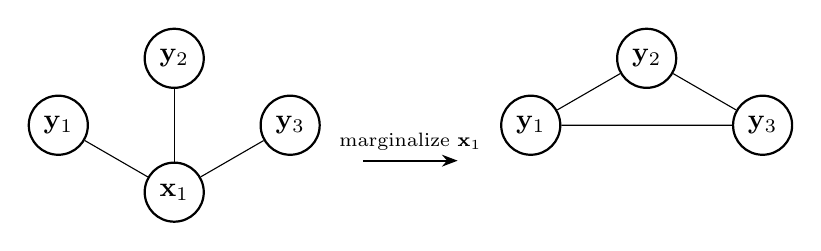
\begin{tikzpicture}
\node[var] (x) at (0,0) {$\bx_1$};
\foreach \n/\a in {1/150,2/90,3/30}{ \node[var] (l\n) at ($(x)+(\a:1.7)$) {$\by_\n$}; \draw (x)--(l\n);}
\draw[->,thick] (2.4,0.4)--(3.6,0.4) node[midway,above,font=\scriptsize]{marginalize $\bx_1$};
\begin{scope}[xshift=6cm]
\foreach \n/\a in {1/150,2/90,3/30}{ \node[var] (m\n) at (\a:1.7) {$\by_\n$};}
\draw (m1)--(m2)--(m3)--(m1);
\end{scope}
\end{tikzpicture}
\caption{Marginalizing a pose that saw three points turns a sparse star into a dense clique: past poses cannot be dropped for free.}
\end{figure}
\begin{intuition}
Filtering throws away the past poses, and the price of forgetting is a dense belief over everything they saw. Graph-based SLAM (next section) keeps the past poses as explicit variables, so the system stays sparse and can be \emph{relinearized}.
\end{intuition}

% =====================================================================
\section{Graph-Based SLAM: Factor Graphs and Least Squares \slr{14--22}}
\subsection{Graph-Based SLAM \slrs{15}}
Graph-based SLAM keeps \emph{every keyframe pose} and represents the problem as a graph. Every node is a camera pose or a map point; every edge is a spatial constraint between two nodes, given by a (uncertain) measurement. Observing a previously seen area creates constraints between non-successive poses. The \textbf{front end} builds the graph from raw data; the \textbf{back end} finds the node configuration that minimizes the error of all constraints.

\begin{figure}[htbp]\centering
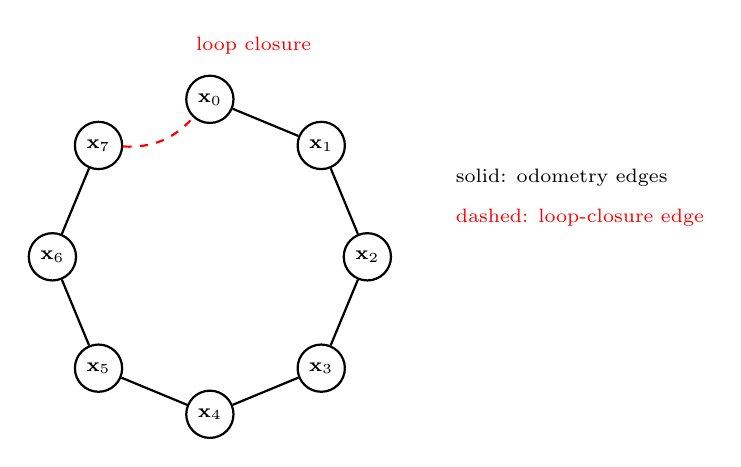
\begin{tikzpicture}
\foreach \i in {0,...,7}{ \node[var,minimum size=6mm] (n\i) at ({90-\i*45}:2) {\scriptsize$\bx_{\i}$};}
\foreach \i/\j in {0/1,1/2,2/3,3/4,4/5,5/6,6/7}{\draw[thick] (n\i)--(n\j);}
\draw[thick,red,dashed] (n7) to[bend right=25] (n0);
\node[font=\scriptsize,red,anchor=south west] at (-0.3,2.45) {loop closure};
\node[font=\scriptsize,anchor=west] at (3.0,1.0) {solid: odometry edges};
\node[font=\scriptsize,anchor=west,red] at (3.0,0.5) {dashed: loop-closure edge};
\end{tikzpicture}
\caption{A pose graph (slide 15): odometry links consecutive poses; recognizing a visited place adds a constraint between non-successive poses.}
\end{figure}

\subsection{Factor Graphs \slrs{16}}
\begin{definition}{Factor graph}{fg}
A \emph{factor graph} is a bipartite graph with \emph{variable} nodes (circles: the unknown poses and points) and \emph{factor} nodes (squares). Each factor $\phi_k$ is joined only to the variables $\Theta_k$ it depends on, and the global function is the product
\[
\phi(\Theta)=\prod_k\phi_k(\Theta_k).
\]
Given the measurements $\mathcal Z$, the posterior is proportional to such a product: $p(\Theta\mid\mathcal Z)\propto\prod_k\phi_k(\Theta_k)$.
\end{definition}

\begin{figure}[htbp]\centering
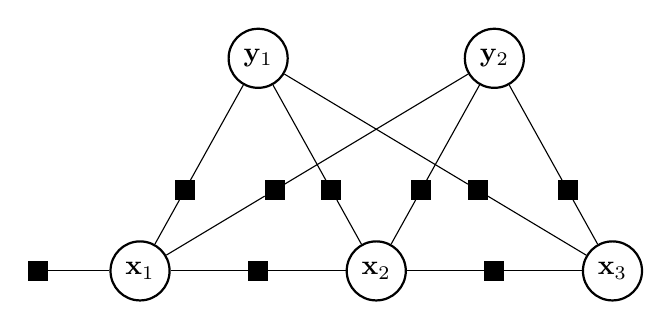
\begin{tikzpicture}
\node[var] (x1) at (0,0) {$\bx_1$}; \node[var] (x2) at (3,0) {$\bx_2$}; \node[var] (x3) at (6,0) {$\bx_3$};
\node[var] (l1) at (1.5,2.7) {$\by_1$}; \node[var] (l2) at (4.5,2.7) {$\by_2$};
\node[fac] (f0) at (-1.3,0) {}; \draw (f0)--(x1);
\node[fac] at (1.5,0) (m12) {}; \draw (x1)--(m12)--(x2);
\node[fac] at (4.5,0) (m23) {}; \draw (x2)--(m23)--(x3);
\foreach \x in {x1,x2,x3}{\foreach \l in {l1,l2}{
 \node[fac] (f\x\l) at ($(\x)!0.38!(\l)$) {}; \draw (\x)--(f\x\l)--(\l);}}
\end{tikzpicture}
\caption{Toy factor graph (redrawn in the spirit of Dellaert and Kaess, Fig.~1.3): three poses, two points, nine factors, namely one prior, two motion factors, and one factor per measurement (six).}
\end{figure}
\begin{intuition}
Think of a factor as ``one piece of evidence'', and its edges as the unknowns it talks about. A GPS reading talks about one pose; an odometry reading about two consecutive poses; a feature observation about one pose and one point. The factor graph is just the table of contents of who-constrains-whom, which will turn out to be exactly the sparsity pattern of the linear system.
\end{intuition}

\subsection{Visual SLAM as a Factor Graph \slrs{17}}
The variables are the camera poses $\bT_i$ and the points $\bX_j$. Each observation adds one \emph{reprojection factor}, a Gaussian on the residual of lecture 05:
\[
\phi_{ij}(\bT_i,\bX_j)\propto\exp\!\Big(-\tfrac12\norm{\mathbf r_{ij}}{\Sigma_{ij}^{-1}}^2\Big),\qquad
\mathbf r_{ij}=\pi(\bT_i\bX_j)-\mathbf u_{ij},
\]
with $\Sigma_{ij}$ the covariance of the pixel noise. A \emph{prior} factor on $\bT_1$ anchors the solution in space; with one camera the scale stays free unless one distance is fixed too (lecture 05). With these Gaussian factors, the most probable variables are the bundle adjustment solution of lecture 05.

\begin{figure}[htbp]\centering
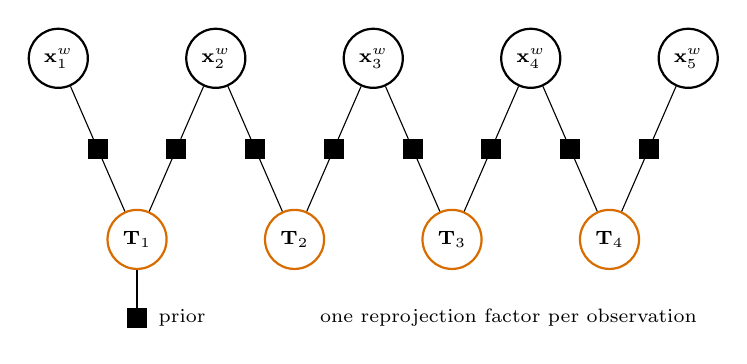
\begin{tikzpicture}
\foreach \j in {1,...,5}{ \node[var] (p\j) at ({2*\j-1},2.3) {\scriptsize$\bx^w_{\j}$};}
\foreach \i in {1,...,4}{ \node[var,draw=orange!85!black,thick] (T\i) at ({2*\i},0) {\scriptsize$\bT_{\i}$};}
\foreach \i in {1,...,4}{ \pgfmathtruncatemacro{\k}{\i+1}
 \node[fac] (a\i) at ($(T\i)!0.5!(p\i)$) {}; \draw (T\i)--(a\i)--(p\i);
 \node[fac] (b\i) at ($(T\i)!0.5!(p\k)$) {}; \draw (T\i)--(b\i)--(p\k);}
\node[fac] (pr) at (2,-1) {}; \draw (T1)--(pr); \node[font=\scriptsize,right] at (2.15,-1) {prior};
\node[font=\scriptsize,anchor=west] at (4.2,-1) {one reprojection factor per observation};
\end{tikzpicture}
\caption{Visual SLAM factor graph (slide 17): each pose sees two neighbouring points.}
\end{figure}

\begin{intuition}
Bundle adjustment is not a different algorithm from SLAM's back end: it is the MAP estimate of this graph. The prior on $\bT_1$ pins the \emph{gauge}: the whole reconstruction could otherwise slide or rotate in space (and, for one camera, scale) with no change in error.
\end{intuition}

\subsection{The Pose Graph \slrs{18}}
The pose graph keeps only the poses. Each edge is a measured \emph{relative pose} between two keyframes $i$ and $j$:
\begin{itemize}[nosep]
\item \textbf{Odometry edge:} between consecutive keyframes, from the motion estimated between them.
\item \textbf{Loop-closure edge:} between non-successive keyframes that observe the same part of the scene, a virtual measurement of keyframe $j$ seen from keyframe $i$.
\end{itemize}
Each edge carries a measured relative pose $\mathbf Z_{ij}$ and an information matrix $\Omega_{ij}$. Eliminating the points exactly would connect every pair of poses that saw a common point (Proposition~\ref{prop:fillin}); the pose graph is kept sparse \emph{by construction}, by using only a selected set of relative-pose edges.

\subsection{From Factors to Least Squares \slrs{19}}
Each factor is a Gaussian in its residual, $\phi_k\propto\exp(-\frac12\be_k^\top\Omega_k\be_k)$.

\begin{theorem}{MAP on a factor graph is nonlinear least squares}{map}
The most probable variables minimize a sum of squared Mahalanobis errors:
\[
\Theta^\star=\argmax_\Theta\prod_k\phi_k(\Theta_k)=\argmin_\Theta\ F(\Theta),\qquad F(\Theta)=\sum_k\be_k(\Theta_k)^\top\Omega_k\,\be_k(\Theta_k),
\]
where $\be_k$ is the residual of factor $k$ (predicted minus actual measurement) and $\Omega_k$ the inverse covariance of the measurement. The sum runs over prior, motion and measurement terms alike.
\end{theorem}
\begin{proof}
$\log\prod_k\phi_k=\sum_k\log\phi_k=\text{const}-\tfrac12\sum_k\be_k^\top\Omega_k\be_k$, and $\log$ is monotone, so maximizing the product is minimizing the sum. \qedhere
\end{proof}
\begin{intuition}
Logs turn products into sums, Gaussians into parabolas. Worked number: two measurements of the same 1D position, $10.0$ with $\sigma=1$ ($\Omega=1$) and $10.6$ with $\sigma=0.5$ ($\Omega=4$). Minimizing $1\,(x-10)^2+4\,(x-10.6)^2$ gives $x=\frac{1\cdot10+4\cdot10.6}{5}=10.48$: the more certain reading pulls four times harder. This is bundle adjustment of lecture 05, \emph{weighted}.
\end{intuition}

\subsection{Error and Information Matrix of an Edge \slrs{20}}
An edge measures the pose of keyframe $j$ seen from keyframe $i$, $\mathbf Z_{ij}$. Since each pose maps world to camera, the poses predict it as $\bT_i\bT_j^{-1}$, which maps camera-$j$ coordinates to camera $i$. The residual compares the two:
\[
\be_{ij}=\log\!\big(\mathbf Z_{ij}^{-1}\,\bT_i\bT_j^{-1}\big)^\vee\in\R^6,\qquad F=\sum_{(i,j)}\be_{ij}^\top\Omega_{ij}\,\be_{ij}.
\]
Here $\mathbf Z_{ij}^{-1}$ maps from $i$ to $j$, so $\be_{ij}=\mathbf 0$ exactly when the poses agree with the measurement; $\Omega_{ij}$ is the inverse covariance of $\mathbf Z_{ij}$ and encodes its uncertainty: the larger $\Omega_{ij}$, the more the edge matters in the optimization.
\begin{intuition}
Think of every edge as a spring whose rest length is the measurement and whose stiffness is $\Omega_{ij}$. Odometry springs are stiff but there are many of them (errors accumulate); a loop-closure spring is softer but connects two far-away parts of the path. Numbers: $\sigma_{\text{odom}}=0.1$\,m gives $\Omega=100$, while $\sigma_{\text{loop}}=1$\,m gives $\Omega=1$: a loop edge is $100\times$ weaker per unit squared error, yet it can still bend a long chain because the chain's accumulated error is spread over hundreds of springs.
\end{intuition}

\subsection{Gauss-Newton on the Pose Graph \slrs{21}}
Around the current poses, every residual is linearized in the increments of lecture 05, $\bT_i\leftarrow\exp(\delta\boldsymbol\xi_i^\wedge)\bT_i$: $\be_{ij}(\mathbf x\boxplus\delta\mathbf x)\approx\be_{ij}+\bJ_{ij}\,\delta\mathbf x$.

\begin{algorithm}{Gauss--Newton / Levenberg--Marquardt on the pose graph}{gn}
Repeat until convergence, starting from a good initial guess (e.g.\ chained odometry):
\begin{enumerate}[nosep]
\item $\bH=\sum_{ij}\bJ_{ij}^\top\Omega_{ij}\bJ_{ij}$, \quad $\bb=\sum_{ij}\bJ_{ij}^\top\Omega_{ij}\be_{ij}$.
\item Solve the normal equations $\bH\,\delta\mathbf x=-\bb$ (Gauss--Newton), or $(\bH+\lambda\bI)\,\delta\mathbf x=-\bb$ (Levenberg--Marquardt).
\item Update $\mathbf x\leftarrow\mathbf x\boxplus\delta\mathbf x$. In LM, the damping $\lambda$ is doubled when a step increases the error and halved otherwise.
\end{enumerate}
\end{algorithm}
\begin{proof}[Derivation of the normal equations]
Substituting the linearization, $F(\mathbf x\boxplus\delta\mathbf x)\approx\sum(\be+\bJ\delta\mathbf x)^\top\Omega(\be+\bJ\delta\mathbf x)=c+2\,\bb^\top\delta\mathbf x+\delta\mathbf x^\top\bH\,\delta\mathbf x$. Setting the gradient $2\bb+2\bH\delta\mathbf x$ to zero gives $\bH\delta\mathbf x=-\bb$. \qedhere
\end{proof}

\begin{proposition}{Gauge freedom}{gauge}
The error $F$ is unchanged if all poses move together, $\bT_i\mapsto\bT_i\mathbf S$ for any rigid $\mathbf S$. Hence $\bH$ is singular (null space of dimension $6$), and the graph is anchored by holding $\bT_1$ fixed, as the prior on the first pose did.
\end{proposition}
\begin{proof}
$(\bT_i\mathbf S)(\bT_j\mathbf S)^{-1}=\bT_i\bT_j^{-1}$, so every $\be_{ij}$ is invariant. Differentiating along the 6-parameter family shows $\bJ\mathbf v=\mathbf 0$ for its tangent directions $\mathbf v$, hence $\bH\mathbf v=\sum\bJ^\top\Omega\bJ\mathbf v=\mathbf 0$. \qedhere
\end{proof}
\begin{intuition}
Pose graphs only know \emph{relative} information, like a map with distances but no coordinates: you can pick the whole thing up and put it down elsewhere. Fixing one pose nails it to the table. LM damping is a safety belt: a large $\lambda$ takes small, gradient-like steps; a small $\lambda$ takes full Gauss--Newton steps. This handles highly non-convex problems better, and loop closures are exactly where the problem is non-convex.
\end{intuition}

\subsection{Sparsity of the Normal Equations \slrs{22}}
A residual depends on $\bT_i$ and $\bT_j$ only, so its Jacobian has two non-zero blocks, $\bJ_{ij}=[\cdots\ \mathbf A_{ij}\ \cdots\ \mathbf B_{ij}\ \cdots]$, and each edge adds to \emph{four blocks of $\bH$ and two of $\bb$}:
\[
\bH_{ii}\mathrel{+}=\mathbf A^\top\Omega\mathbf A,\ \ \bH_{ij}\mathrel{+}=\mathbf A^\top\Omega\mathbf B,\ \ \bH_{ji}\mathrel{+}=\mathbf B^\top\Omega\mathbf A,\ \ \bH_{jj}\mathrel{+}=\mathbf B^\top\Omega\mathbf B,\qquad
\bb_i\mathrel{+}=\mathbf A^\top\Omega\be,\ \ \bb_j\mathrel{+}=\mathbf B^\top\Omega\be.
\]
\begin{proposition}{Sparsity pattern of $\bH$}{sparse}
The block $\bH_{ij}$ is non-zero if and only if there is an edge between $i$ and $j$. The block pattern of $\bH$ is therefore the adjacency matrix of the graph plus the diagonal, and $\bH$ is assembled by summing the contribution of each edge.
\end{proposition}
\begin{proof}
Off-diagonal blocks only receive the terms $\mathbf A^\top\Omega\mathbf B$ above, one per edge joining $i$ and $j$; all other products $\bJ_{kl}^\top\Omega\bJ_{kl}$ are zero in block $(i,j)$. \qedhere
\end{proof}
\begin{figure}[htbp]\centering
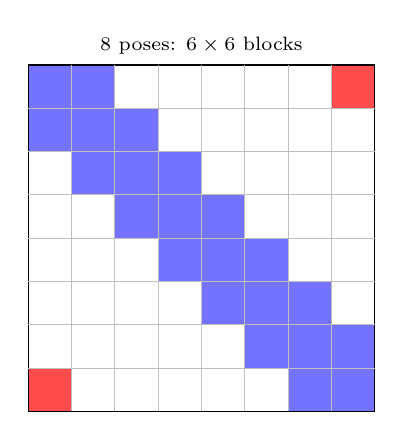
\begin{tikzpicture}[scale=0.55]
\foreach \i in {1,...,8}{\foreach \j in {1,...,8}{
  \pgfmathtruncatemacro{\d}{abs(\i-\j)}
  \ifnum\d<2 \fill[blue!55] (\j-1,-\i) rectangle (\j,-\i+1);\fi
}}
\fill[red!70] (7,-1) rectangle (8,0); \fill[red!70] (0,-8) rectangle (1,-7);
\draw (0,0) rectangle (8,-8);
\foreach \k in {1,...,7}{\draw[gray!50] (\k,0)--(\k,-8); \draw[gray!50] (0,-\k)--(8,-\k);}
\node[font=\scriptsize] at (4,0.45) {8 poses: $6\times6$ blocks};
\end{tikzpicture}
\caption{Block sparsity of $\bH$ for the ring pose graph of slide 15: diagonal and first off-diagonals come from odometry (blue), the two red blocks come from the single loop closure.}
\end{figure}
\begin{intuition}
Worked numbers: $1000$ poses with $6$ degrees of freedom give $\bH\in\R^{6000\times6000}$, i.e.\ $36$ million entries if dense. But there are only about $1000$ diagonal and $2\times999$ off-diagonal blocks of $36$ numbers, roughly $108{,}000$ non-zeros ($0.3\%$). Sparse solvers (sparse Cholesky, conjugate gradients) exploit this, which is why graph-based SLAM scales to the 11\,km running example while a dense EKF covariance cannot.
\end{intuition}

% =====================================================================
\section{The Visual SLAM Pipeline: ORB-SLAM \slr{23--32}}
\subsection{Pipeline Overview \slrs{24}}
\textbf{ORB-SLAM}, a keyframe-based monocular SLAM system, runs three threads in parallel: \textbf{tracking} localizes the camera at every frame and decides when to insert a keyframe; \textbf{local mapping} processes each new keyframe and runs bundle adjustment around it; \textbf{loop closing} searches for a loop at every keyframe and corrects the drift by pose graph optimization. The \emph{front end} abstracts the images into features and data associations; the \emph{back end} estimates the variables from them (Section~6.3).

\begin{figure}[htbp]\centering
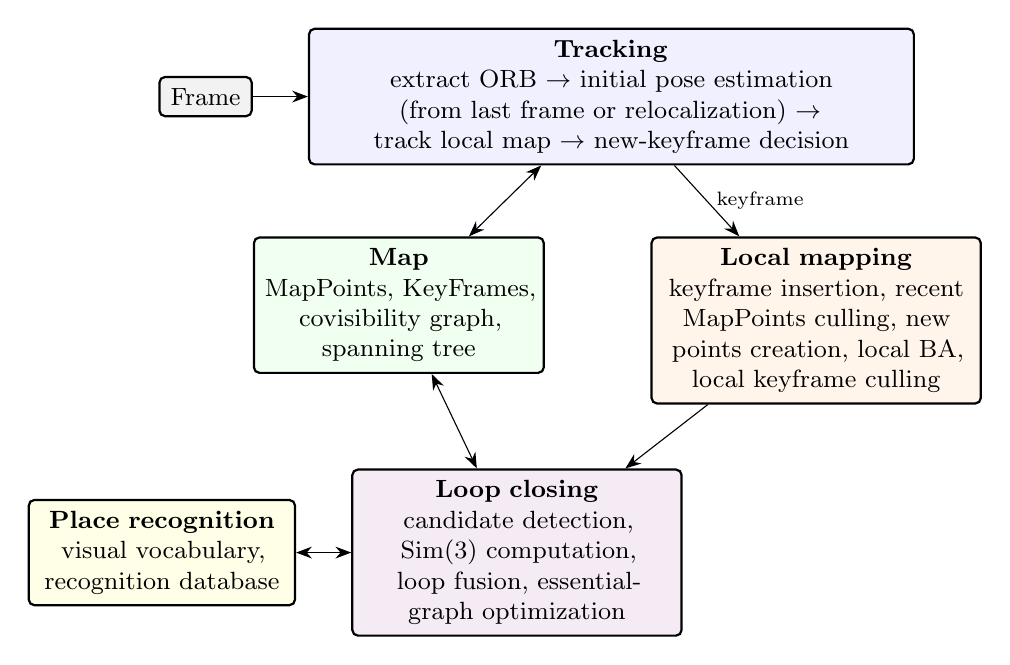
\begin{tikzpicture}[node distance=5mm]
\node[blk,fill=blue!6,text width=7.4cm] (trk) {\textbf{Tracking}\\ extract ORB $\to$ initial pose estimation (from last frame or relocalization) $\to$ track local map $\to$ new-keyframe decision};
\node[blk,fill=gray!10,left=of trk,xshift=-2mm] (fr) {Frame};
\node[blk,fill=green!6,below=9mm of trk,text width=3.4cm,xshift=-2.7cm] (map) {\textbf{Map}\\ MapPoints, KeyFrames, covisibility graph, spanning tree};
\node[blk,fill=orange!8,below=9mm of trk,text width=3.9cm,xshift=2.6cm] (lm) {\textbf{Local mapping}\\ keyframe insertion, recent MapPoints culling, new points creation, local BA, local keyframe culling};
\node[blk,fill=violet!8,below=8mm of map,text width=3.9cm,xshift=1.5cm,yshift=-4mm] (lc) {\textbf{Loop closing}\\ candidate detection, Sim(3) computation, loop fusion, essential-graph optimization};
\node[blk,fill=yellow!10,left=of lc,text width=3.1cm,xshift=-2mm] (pr) {\textbf{Place recognition}\\ visual vocabulary, recognition database};
\draw[->] (fr)--(trk);
\draw[<->] (trk)--(map);
\draw[->] (trk)--(lm) node[midway,right,font=\scriptsize]{keyframe};
\draw[->] (lm)--(lc);
\draw[<->] (pr)--(lc);
\draw[<->] (lc)--(map);
\end{tikzpicture}
\caption{ORB-SLAM threads and data structures (redrawn from the slide 24 block diagram).}
\end{figure}

\begin{figure}[htbp]\centering
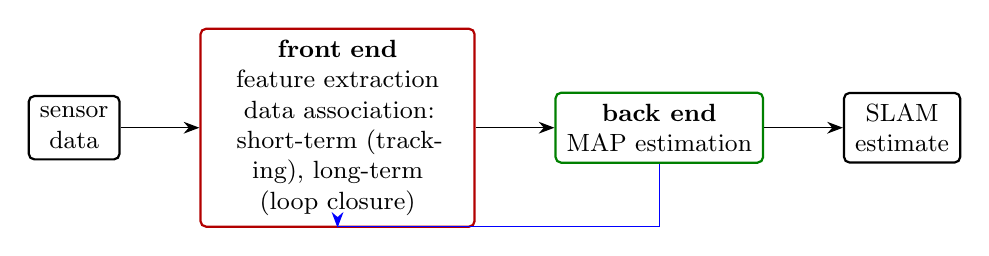
\begin{tikzpicture}
\node[blk] (s) {sensor\\data};
\node[blk,right=10mm of s,draw=red!70!black,text width=3.2cm] (fe) {\textbf{front end}\\ feature extraction\\ data association: short-term (tracking), long-term (loop closure)};
\node[blk,right=10mm of fe,draw=green!50!black] (be) {\textbf{back end}\\ MAP estimation};
\node[blk,right=10mm of be] (est) {SLAM\\estimate};
\draw[->] (s)--(fe); \draw[->] (fe)--(be); \draw[->] (be)--(est);
\draw[->,blue] (be.south) -- ++(0,-0.8) -| (fe.south);
\end{tikzpicture}
\caption{Front end / back end split (slide 24, right): the back end also feeds predictions back to guide data association.}
\end{figure}
\begin{intuition}
The split mirrors the lecture: Section 6.3 was the back end (sparse least squares, assumed data associations), and this section is a front end that produces those associations fast enough for 30 frames per second. Three threads exist because the three jobs have different deadlines: tracking must finish within one frame, local mapping within a keyframe interval, loop closing can take longer.
\end{intuition}

\subsection{ORB Features and Matching \slrs{25}}
ORB-SLAM uses the same features for tracking, mapping, relocalization and loop detection. As in lecture 05, a feature is a keypoint with a descriptor.
\begin{itemize}[nosep]
\item Extraction must take much less than the 33\,ms between frames, which excludes SIFT at about 300\,ms.
\item \textbf{ORB}: corners from the FAST detector, given an orientation, found at 8 scale levels a factor 1.2 apart, each with a binary descriptor; the orientation makes it rotation invariant.
\item 1000 keypoints per image up to $752\times480$ pixels, 2000 on larger images ($1241\times376$), spread over a grid.
\end{itemize}
\begin{definition}{Hamming distance}{hamming}
For binary descriptors $\mathbf d,\mathbf d'\in\{0,1\}^n$ the \emph{Hamming distance} is the number of differing bits, $\|\mathbf d\oplus\mathbf d'\|_1=\mathrm{popcount}(\mathbf d\ \mathrm{XOR}\ \mathbf d')$.
\end{definition}
\begin{intuition}
Matching two descriptors is one XOR and one popcount instruction: orders of magnitude cheaper than the Euclidean distance between 128 floats of SIFT. Example with 8 bits: \texttt{10110010} vs.\ \texttt{10011010} differ in $2$ positions, so $d=2$. The 8-level pyramid with factor $1.2$ covers a total scale range of $1.2^7\approx3.6$, which is why ORB matches survive strong zoom changes.
\end{intuition}
\imgph[4.2cm]{25}{ORB matches between a frame and a keyframe under a strong change of scale.}

\subsection{Map Initialization \slrs{26}}
The first map needs the relative pose of two frames and triangulated points, for planar and general scenes alike. Between a reference frame 1 and the current frame 2, two models are fitted in parallel with RANSAC: a homography $\mathbf x_2\simeq\bH_{21}\mathbf x_1$ (4 points, planar scene) and a fundamental matrix $\mathbf x_2^\top\mathbf F_{21}\mathbf x_1=0$ (8 points, general scene), each scored by its symmetric transfer error
\[
S_M=\sum_i\Big[\rho_M\big(d^2(\mathbf x_1^i,M^{-1}\mathbf x_2^i)\big)+\rho_M\big(d^2(\mathbf x_2^i,M\mathbf x_1^i)\big)\Big].
\]
\begin{algorithm}{ORB-SLAM map initialization}{init}
\begin{enumerate}[nosep]
\item Fit $\bH_{21}$ and $\mathbf F_{21}$ with RANSAC and compute the scores $S_H$, $S_F$.
\item Select the homography if $S_H/(S_H+S_F)>0.45$ (planar scenes and low parallax); otherwise the fundamental matrix.
\item Recover the motion hypotheses: 8 from the essential matrix or 4 from the homography (lecture 05); triangulate with all of them.
\item If there is no clear winner, \emph{create no map} and try with new frames.
\item Refine the first map by full bundle adjustment; its scale is arbitrary (lecture 05).
\end{enumerate}
\end{algorithm}
\begin{intuition}
A homography explains almost anything seen with \emph{no parallax} (a plane, or pure rotation), but then depth is ill-defined and triangulation is unreliable. ORB-SLAM prefers to \emph{wait for parallax} rather than start from a wrong planar map; the slide shows two other systems that started wrongly and drifted, while ORB-SLAM, which waited, did not.
\end{intuition}
\imgph[5.2cm]{26}{Some time after initialization: two other systems (top, middle) started from a wrong planar map; ORB-SLAM (bottom) waited for parallax.}

\subsection{Tracking \slrs{27}}
The tracking thread estimates the pose of every frame:
\begin{enumerate}[nosep]
\item \textbf{Prediction:} a constant-velocity motion model, $\bT_t^{\text{pred}}=(\bT_{t-1}\bT_{t-2}^{-1})\,\bT_{t-1}$, predicts the pose and guides the search for the points seen in the last frame; if too few are found, a wider search follows.
\item \textbf{Local map:} the keyframes that share points with the frame, and their covisible neighbours; their points are projected into the frame and matched near the projection, at the predicted scale.
\item \textbf{Motion-only bundle adjustment:} the reprojection error of lecture 05 over the pose alone, points fixed, with a robust (Huber) cost,
\[
\bT^\star=\argmin_{\bT}\sum_{j}\rho_{\text{Huber}}\!\Big(\norm{\mathbf u_j-\pi(\bT\bX_j)}{\Sigma^{-1}}^2\Big).
\]
\end{enumerate}
\begin{intuition}
Only $6$ unknowns are optimized, so this runs in a few milliseconds per frame. The Huber cost behaves quadratically for small errors and linearly for large ones, so one wrong match (an outlier with a 50-pixel error) cannot dominate $100$ good ones. \textbf{PTAM}, a monocular system for small augmented-reality workspaces, predicts with a decaying velocity and tracks coarse to fine: 50 points at the coarsest image scale, then up to 1000.
\end{intuition}
\imgph[4.8cm]{27}{Keyframes (blue), current camera (green), map points (black) and local map (red).}

\subsection{Keyframes \slrs{28}}
PTAM splits SLAM into two threads that run in parallel: \textbf{tracking} processes every frame in real time (freed from updating the map, it can process each image more thoroughly), and \textbf{mapping} works on keyframes only: many video frames are redundant, and a smaller set of useful keyframes is refined by bundle adjustment without strict real-time limits.
\begin{itemize}[nosep]
\item PTAM: a frame becomes a keyframe if tracking is good, more than twenty frames have passed, and the camera is a minimum distance (set by the mean scene depth) from the existing keyframes.
\item ORB-SLAM instead inserts keyframes \emph{as fast as possible}, which keeps tracking robust to rotations, and culls the redundant ones in local mapping.
\end{itemize}
\begin{intuition}
Keyframes are the ``postcards'' of the trip: you do not keep every frame of a 30\,Hz video (11\,km would be hundreds of thousands), only enough views to triangulate the scene. ORB-SLAM's strategy is generous insertion followed by pruning: it is easier to remove a redundant postcard than to recover a view you never kept.
\end{intuition}
\imgph[5cm]{28}{A desk mapped by PTAM: two views of the map with its keyframes (top), and the 57 keyframes (bottom).}

\subsection{Local Mapping \slrs{29}}
\begin{definition}{Covisibility graph}{covis}
Nodes are keyframes; an edge joins two keyframes that share at least $15$ map points, weighted by the number of shared points.
\end{definition}
For every new keyframe the local mapping thread:
\begin{enumerate}[nosep]
\item inserts it in the covisibility graph;
\item culls recent points: a point stays only if it is found in more than $25\%$ of the frames predicted to see it, and from at least three keyframes;
\item triangulates new points from unmatched features in covisible keyframes, checking depth, parallax, reprojection error and scale;
\item runs \textbf{local bundle adjustment} on the keyframe, its covisible keyframes and all their points; the other keyframes that see these points stay fixed;
\item culls redundant keyframes, whose points are $90\%$ seen by at least three other keyframes.
\end{enumerate}
\begin{figure}[htbp]\centering
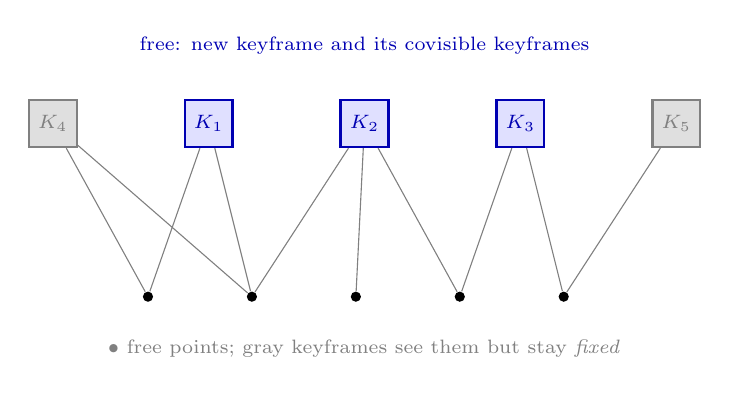
\begin{tikzpicture}[scale=1.1]
\foreach \i/\x in {1/0,2/1.8,3/3.6}{ \node[draw,blue!70!black,fill=blue!12,thick,minimum size=6mm] (k\i) at (\x,2) {\scriptsize$K_{\i}$};}
\foreach \i/\x in {4/-1.8,5/5.4}{ \node[draw,gray,fill=gray!25,thick,minimum size=6mm] (k\i) at (\x,2) {\scriptsize$K_{\i}$};}
\foreach \j/\x in {1/-0.7,2/0.5,3/1.7,4/2.9,5/4.1}{ \node[circle,fill=black,inner sep=1.3pt] (q\j) at (\x,0) {};}
\foreach \a/\b in {k1/q1,k1/q2,k2/q2,k2/q3,k2/q4,k3/q4,k3/q5,k4/q1,k5/q5,k4/q2}{\draw[gray] (\a)--(\b);}
\node[font=\scriptsize,blue!70!black] at (1.8,2.9) {free: new keyframe and its covisible keyframes};
\node[font=\scriptsize,gray] at (1.8,-0.6) {$\bullet$ free points; gray keyframes see them but stay \emph{fixed}};
\end{tikzpicture}
\caption{Local bundle adjustment (slide 29, step 4): only a small neighbourhood is optimized; fixed keyframes anchor it to the rest of the map.}
\end{figure}
\begin{intuition}
The covisibility graph answers ``who looks at the same things as me?''. Optimizing only that neighbourhood keeps the cost bounded while the map grows to kilometres: \emph{local} BA is constant-time per keyframe, unlike EKF-SLAM whose cost grows with the whole map. Fixing the outer keyframes plays the role of the prior on $\bT_1$ for the local problem.
\end{intuition}
\imgph[5cm]{29}{Covisibility graph of an indoor handheld sequence (TUM RGB-D).}

\subsection{Loop Detection with Bags of Binary Words \slrs{30}}
A loop is detected by \emph{appearance}: each image is compared with all the past ones, fast enough for every frame.
\begin{itemize}[nosep]
\item \textbf{Vocabulary:} binary descriptors clustered offline into a tree of $10$ branches and $6$ levels whose leaves are the visual words; an image becomes a vector of word weights.
\item \textbf{Inverse index:} for each word, the images that contain it, so a query visits only images sharing words with it.
\item \textbf{Checks:} the score is normalized by that of the previous image; a match must agree with previous matches and be supported by a fundamental matrix with at least $12$ RANSAC inliers.
\item ORB-SLAM uses ORB words, groups candidates by covisibility rather than by time, and accepts a loop after three consecutive consistent candidates. $21.6$\,ms per image on average, over $26292$ images.
\end{itemize}
\begin{proposition}{Why a hierarchical vocabulary is fast}{vocab}
A tree with branching factor $k$ and $L$ levels has $k^L$ leaves (words), but quantizing a descriptor needs only $kL$ comparisons.
\end{proposition}
\begin{proof}
At each level the descriptor is compared with the $k$ children of the current node and descends into the closest one; there are $L$ levels. \qedhere
\end{proof}
\begin{figure}[htbp]\centering
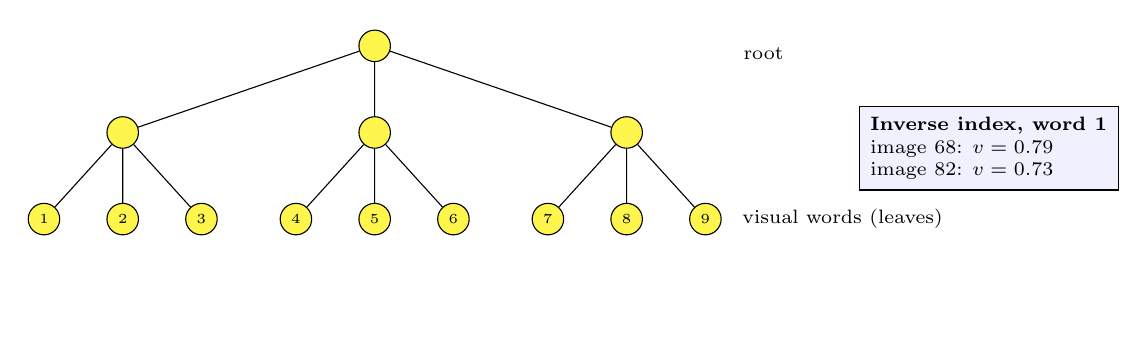
\begin{tikzpicture}[level distance=1.1cm,
  level 1/.style={sibling distance=3.2cm},level 2/.style={sibling distance=1cm},
  every node/.style={circle,draw,fill=yellow!70,inner sep=1.5pt,minimum size=4mm,font=\tiny}]
\node {} child {node {} child {node{1}} child {node{2}} child {node{3}}}
 child {node {} child {node{4}} child {node{5}} child {node{6}}}
 child {node {} child {node{7}} child {node{8}} child {node{9}}};
\node[draw=none,fill=none,font=\scriptsize,anchor=west] at (4.6,-0.1) {root};
\node[draw=none,fill=none,font=\scriptsize,anchor=west] at (4.6,-2.2) {visual words (leaves)};
\node[rectangle,draw,rounded corners=0pt,fill=blue!6,font=\scriptsize,align=left,inner sep=4pt,minimum size=0pt] at (7.8,-1.3)
 {\textbf{Inverse index, word 1}\\ image 68: $v=0.79$\\ image 82: $v=0.73$};
\end{tikzpicture}
\caption{Vocabulary tree and inverse index (slide 30; the sketch shows $k=3,\ L=2$, the system uses $k=10,\ L=6$).}
\end{figure}
\begin{intuition}
Numbers: $10$ branches and $6$ levels give $10^6=1{,}000{,}000$ words, but a descriptor is quantized with only $10\times6=60$ comparisons. The inverse index is the book index idea: to find pages about ``Cholesky'' you do not read the whole book. Normalizing by the score of the previous image avoids false alarms in places that simply look similar to everything (corridors). The score between two images lies between $0$ and $1$.
\end{intuition}

\subsection{Loop Correction and Scale Drift \slrs{31}}
One camera cannot observe scale, so the scale drifts too: a monocular map drifts in \textbf{seven} degrees of freedom (rotation, translation and scale). A pose graph over $\SE$ closes the loop but \emph{keeps the scale drift}. The poses become similarities (lecture 01).
\begin{definition}{Similarity transformation $\Sim$}{sim3}
$\mathbf S=\begin{pmatrix}s\mathbf R&\mathbf t\\\mathbf 0^\top&1\end{pmatrix}$, with $\mathbf R\in SO(3)$, $\mathbf t\in\R^3$, $s>0$; it acts on points as $\bX\mapsto s\mathbf R\bX+\mathbf t$ and has $7$ degrees of freedom. The pose-graph residual has the same form as before, $\be_{ij}=\log(\mathbf Z_{ij}^{-1}\mathbf S_i\mathbf S_j^{-1})^\vee\in\R^7$.
\end{definition}
\begin{itemize}[nosep]
\item Odometry edges keep their measured motion with scale $1$; the loop edge carries the measured change of scale.
\item \textbf{ORB-SLAM:} the loop similarity comes from 3D--3D point matches, by RANSAC and Horn's method; duplicated points are fused; the pose graph over $\Sim$ is optimized on the \emph{essential graph}: a spanning tree, the covisibility edges with at least $100$ shared points, and the loop edges.
\end{itemize}
\begin{figure}[htbp]\centering
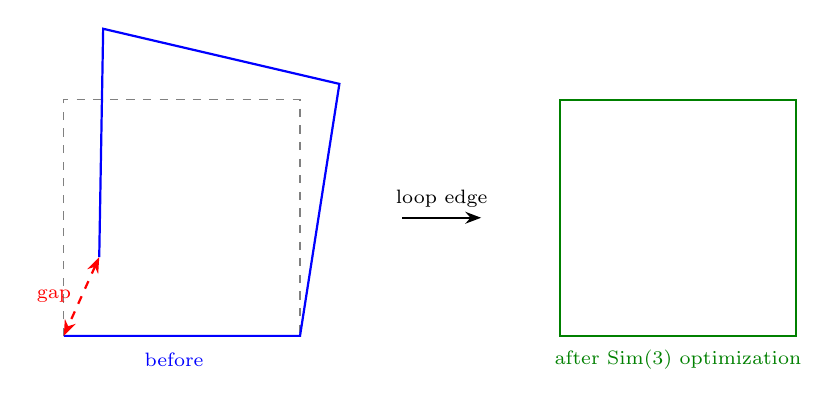
\begin{tikzpicture}[scale=1.0]
\draw[dashed,gray] (0,0) rectangle (3,3);
\draw[thick,blue] (0,0)--(3,0)--(3.5,3.2)--(0.5,3.9)--(0.45,1.0);
\node[blue,font=\scriptsize] at (1.4,-0.3) {before};
\draw[red,thick,dashed,<->] (0.45,1.0)--(0,0) node[midway,left,font=\scriptsize]{gap};
\draw[->,thick] (4.3,1.5)--(5.3,1.5) node[midway,above,font=\scriptsize]{loop edge};
\begin{scope}[xshift=6.3cm]
\draw[thick,green!50!black] (0,0) rectangle (3,3);
\node[green!50!black,font=\scriptsize] at (1.5,-0.3) {after $\Sim$ optimization};
\end{scope}
\end{tikzpicture}
\caption{Loop closure (sketch of the slide 31 experiment): drift in rotation, translation and scale leaves the loop open; the loop edge and its scale are distributed along the cycle.}
\end{figure}
\begin{intuition}
Numbers: if after a loop the end of the trajectory is estimated at relative scale $1.10$ with respect to the start, the loop edge says so, and the $\Sim$ optimization spreads $\ln1.10\approx0.0953$ over, say, $100$ keyframes, about $0.00095$ of log-scale each. A $\SE$ optimization has no scale variable, so it can bend the path but the scale error stays: the slide shows the 6\,DoF result still distorted while the 7\,DoF result matches the aerial photo.
\end{intuition}
\imgph[6.2cm]{31}{A square circled by a hand-held camera: (a) before optimization, (b) over $\SE$ (6\,DoF), (c) over $\Sim$ (7\,DoF), (d) aerial photo.}

\subsection{Relocalization \slrs{32}}
When tracking is lost, after an occlusion or an abrupt motion, the camera is localized again in the existing map:
\begin{enumerate}[nosep]
\item the frame is converted into a bag of words, and the place recognition database returns candidate keyframes;
\item for each candidate, ORB features are matched to its map points, and RANSAC with PnP (lecture 05) estimates a camera pose;
\item a pose with enough inliers is refined and guides the search for more matches; with enough inliers, tracking resumes.
\end{enumerate}
On indoor handheld sequences with ground truth (TUM RGB-D), $78.4\%$ of $2769$ frames are relocalized in a map built from the first 30\,s; with people walking through the scene, $77.9\%$ of $859$ frames.
\begin{intuition}
Relocalization reuses everything already built: the same bag-of-words database that detects loops here answers ``where am I?'' from a single image. It is a \emph{global} localization problem (no prior pose), solved by PnP inside RANSAC, which tolerates the moving people that spoil many of the matches.
\end{intuition}
\imgph[4.2cm]{32}{A relocalization among moving people: ORB matches between the frame and a keyframe.}

% =====================================================================
\section{Research Directions \slr{33--40}}
\subsection{Continuous Time: Rolling-Shutter Cameras \slrs{34}}
A rolling-shutter camera exposes every line of the image for a different period, each one more delayed than the last. When the camera moves during the exposure, the image appears distorted and skewed. So far every image had one pose, as with a global shutter, where all pixels are exposed over the same duration. Earlier work removed the distortion first, to recreate a global-shutter image. On a simulated monocular sequence, the loop-closure position error is $0.0472$ of the distance travelled when time is modelled as for a global shutter, and $0.0057$ when the rolling shutter is modelled.
\begin{intuition}
The numbers: $4.7\%$ versus $0.57\%$ of the path length, an $8\times$ reduction ($0.0472/0.0057\approx8.3$) just from admitting that the rows of an image are taken at different times. Each scanline is a tiny camera with its own timestamp, so the \emph{trajectory}, not a pose per image, becomes the unknown.
\end{intuition}
\begin{figure}[htbp]\centering
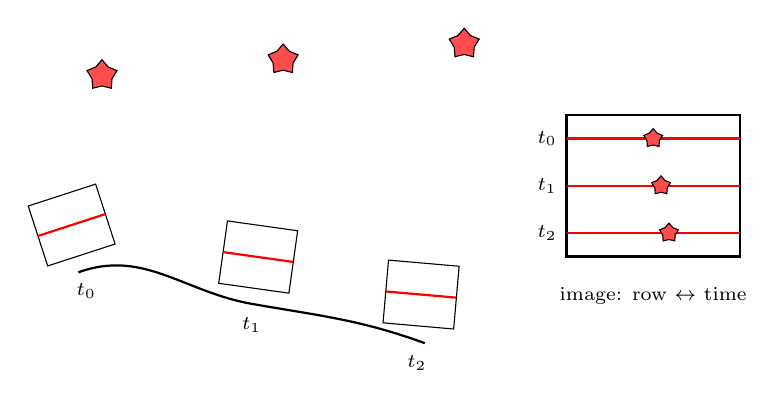
\begin{tikzpicture}[scale=1.0]
\draw[thick] (0,0) to[out=20,in=170] (2.2,-0.4) to[out=-10,in=160] (4.4,-0.9);
\foreach \i/\x/\y/\r in {0/0.1/0.03/18,1/2.2/-0.4/-8,2/4.3/-0.88/-5}{
 \draw[rotate around={\r:(\x,\y)},fill=white] (\x-0.45,\y+0.2) rectangle (\x+0.45,\y+1.0);
 \draw[rotate around={\r:(\x,\y)},thick,red] (\x-0.45,\y+0.6) -- (\x+0.45,\y+0.6);
 \node[font=\scriptsize,below] at (\x,\y-0.05) {$t_{\i}$};
 \node[star5,fill=red!70] at (\x+0.2*\i+0.2,2.5+0.2*\i) {};}
\draw[thick] (6.2,0.2) rectangle (8.4,2.0);
\foreach \i/\yy in {0/1.7,1/1.1,2/0.5}{ \draw[red,thick] (6.2,\yy)--(8.4,\yy); \node[font=\scriptsize,left] at (6.2,\yy) {$t_{\i}$};
 \node[star5,fill=red!70,minimum size=2.5mm] at (7.3+0.1*\i,\yy) {};}
\node[font=\scriptsize] at (7.3,-0.3) {image: row $\leftrightarrow$ time};
\end{tikzpicture}
\caption{Each scanline is a camera with its own time along the trajectory (redrawn from slide 34); together they form the image.}
\end{figure}
\imgph[3.8cm]{34}{A rolling-shutter warp (distorted and skewed building facade).}

\subsection{Continuous Time: Cumulative B-Splines on $\SE$ \slrs{35}}
The trajectory becomes a continuous function of time, a \emph{cumulative cubic B-spline} built with the Lie algebra (lecture 05). Control poses $\bT_i$ sit at uniform times $t_i$, $\Delta t$ apart. For $t\in[t_i,t_{i+1})$ let $u=(t-t_i)/\Delta t\in[0,1)$; the four poses $\bT_{i-1},\dots,\bT_{i+2}$ give
\[
\bT(t)=\exp\!\big(\tilde B_3(u)\,\boldsymbol\delta_3\big)\exp\!\big(\tilde B_2(u)\,\boldsymbol\delta_2\big)\exp\!\big(\tilde B_1(u)\,\boldsymbol\delta_1\big)\,\bT_{i-1},\qquad
\boldsymbol\delta_j=\log\!\big(\bT_{i-1+j}\bT_{i-2+j}^{-1}\big),
\]
with cumulative basis functions
\[
\tilde B_1=\tfrac16(5+3u-3u^2+u^3),\quad \tilde B_2=\tfrac16(1+3u+3u^2-2u^3),\quad \tilde B_3=\tfrac16u^3 .
\]
(Spline written for world-to-camera poses with left-multiplied increments.) $\boldsymbol\delta_j$ is the increment from control pose $j-1$ to $j$, and the trajectory is twice continuously differentiable. Each pixel is projected with the pose at its own time: a point on image row $v$ is observed at $t=t_0+\frac{v}{h}\,t_{\text{ro}}$, $h$ being the image height and $t_{\text{ro}}$ the frame readout time. The control poses are the unknowns of the least squares, optimized over a sliding window.
\begin{figure}[htbp]\centering
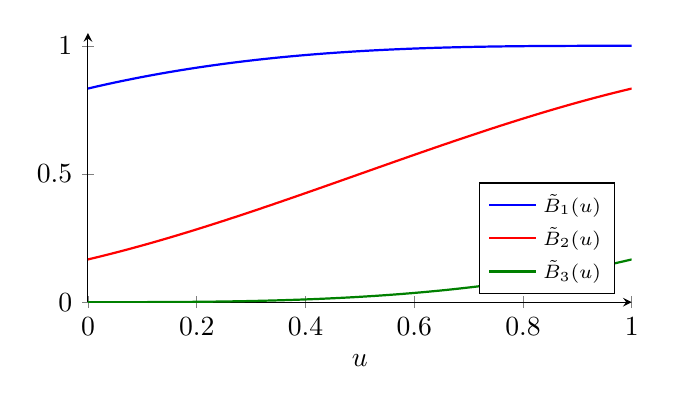
\begin{tikzpicture}
\begin{axis}[width=0.7\linewidth,height=5cm,xlabel={$u$},ymin=0,ymax=1.05,xmin=0,xmax=1,domain=0:1,samples=60,no markers,axis lines=left,legend pos=south east,legend style={font=\scriptsize}]
\addplot[blue,thick]{(5+3*x-3*x^2+x^3)/6}; \addlegendentry{$\tilde B_1(u)$}
\addplot[red,thick]{(1+3*x+3*x^2-2*x^3)/6}; \addlegendentry{$\tilde B_2(u)$}
\addplot[green!50!black,thick]{x^3/6}; \addlegendentry{$\tilde B_3(u)$}
\end{axis}
\end{tikzpicture}
\caption{Cumulative cubic B-spline basis functions: at $u=0$ the weights are $(5/6,1/6,0)$ and at $u=1$ they are $(1,5/6,1/6)$, which equals the $u=0$ weights of the next interval after shifting the control poses by one, so the curve is continuous.}
\end{figure}
\begin{intuition}
A spline is a flexible ruler pinned at control poses: you do not store a pose per row, only a handful of control poses per window, and any timestamp inside gives a smooth pose. Advantage: IMU, rolling-shutter and event-camera measurements at arbitrary timestamps can all be written as functions of the same few unknowns. Further reading: a survey of continuous-time state estimation in robotics (splines and Gaussian processes), Talbot et al., T-RO 2025.
\end{intuition}

\subsection{Active SLAM \slrs{36}}
SLAM is \emph{passive}: it does not guide the motion. \textbf{Active SLAM} plans and controls the motion of the robot to build the most accurate and complete model of the environment. It is a decision between two opposite goals, exploring new areas or revisiting those already seen (the \emph{exploration--exploitation dilemma}). With high uncertainty, places where a loop could close carry more information than new frontiers.
\begin{algorithm}{Active SLAM loop}{active}
Repeat until a stopping condition is met: (1) identify candidate actions; (2) compute the utility of each; (3) select and execute the best.
\end{algorithm}
The utility is the expected uncertainty of the pose and the map. For a Gaussian belief whose covariance $\Sigma\in\R^{n\times n}$ has eigenvalues $\lambda_1,\dots,\lambda_n$, the \emph{D-optimality} criterion measures the volume of the uncertainty ellipsoid,
\[
\text{D-opt}(\Sigma)=\exp\!\Big(\tfrac1n\sum_{k=1}^n\log\lambda_k\Big)=\det(\Sigma)^{1/n},
\]
to be minimized.
\begin{intuition}
Worked number: eigenvalues $(4,1)$ give $\det^{1/2}=2$; after an informative view that shrinks the long axis to $(1,1)$ the criterion is $1$. The geometric mean of the eigenvalues is used because it rewards shrinking \emph{any} axis, not only the largest one.
\end{intuition}
\begin{figure}[htbp]\centering
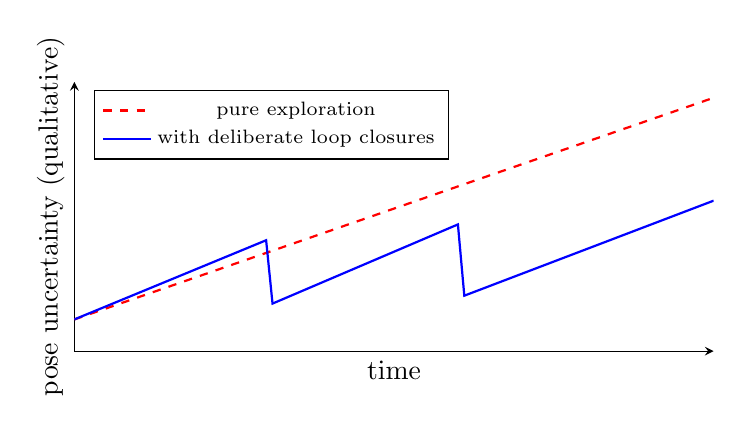
\begin{tikzpicture}
\begin{axis}[width=0.8\linewidth,height=5cm,xlabel={time},ylabel={pose uncertainty (qualitative)},ymin=0,ymax=3.4,xmin=0,xmax=10,axis lines=left,ticks=none,legend pos=north west,legend style={font=\scriptsize}]
\addplot[red,thick,dashed] coordinates{(0,0.4)(10,3.2)}; \addlegendentry{pure exploration}
\addplot[blue,thick] coordinates{(0,0.4)(3,1.4)(3.1,0.6)(6,1.6)(6.1,0.7)(10,1.9)}; \addlegendentry{with deliberate loop closures}
\end{axis}
\end{tikzpicture}
\caption{Exploration--exploitation (qualitative sketch): exploring grows uncertainty; revisiting a known place closes a loop and resets it.}
\end{figure}

\subsection{Active SLAM with an Active Stereo Head \slrs{37}}
The work that named active SLAM: a wheeled robot carries a stereo head with four degrees of freedom. An EKF estimates the robot and a map of point features, and the head fixates one feature at a time; it decides where to look, not where to move. For each visible feature $i$ the EKF predicts the measurement and its innovation covariance $\bS_i$. The head fixates the feature whose position is hardest to predict, the one with the largest $3\sigma$ ellipsoid:
\[
i^\star=\argmax_i\ \mathrm{Vol}_{3\sigma}(\bS_i)=\argmax_i\ \det(\bS_i)^{1/2}.
\]
\begin{intuition}
It is MonoSLAM's search ellipse turned into a decision: look at the thing you are \emph{least sure about}, because a measurement there reduces uncertainty the most. The ellipsoid volume is $\tfrac43\pi\,3^3\sqrt{\det\bS_i}$ for a 3D innovation, so ranking by $\det\bS_i$ is the same as ranking by volume.
\end{intuition}
\imgph[4.2cm]{37}{The robot and its active head (top); fixated views of features 0, 5, 11, 12 and 14, each marked by a white square (bottom).}

\subsection{Active Localization: Learning Where to Look \slrs{38}}
\textbf{Active localization} chooses where the camera should look so that it localizes accurately in a known map, built by structure-from-motion.
\begin{figure}[htbp]\centering
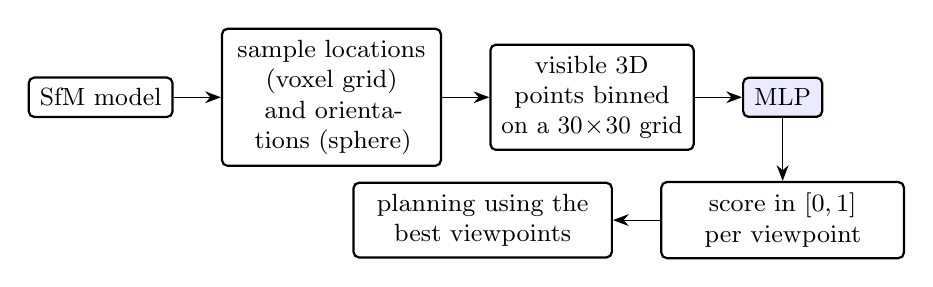
\begin{tikzpicture}[node distance=6mm]
\node[blk] (sfm) {SfM model};
\node[blk,right=of sfm,text width=2.5cm] (samp) {sample locations (voxel grid) and orientations (sphere)};
\node[blk,right=of samp,text width=2.3cm] (enc) {visible 3D points binned on a $30\times30$ grid};
\node[blk,right=of enc,fill=blue!8] (mlp) {MLP};
\node[blk,below=8mm of mlp,text width=2.8cm] (sc) {score in $[0,1]$ per viewpoint};
\node[blk,left=of sc,text width=3cm] (pl) {planning using the best viewpoints};
\draw[->] (sfm)--(samp); \draw[->] (samp)--(enc); \draw[->] (enc)--(mlp); \draw[->] (mlp)--(sc); \draw[->] (sc)--(pl);
\end{tikzpicture}
\caption{Active localization pipeline (redrawn from slide 38).}
\end{figure}
\begin{itemize}[nosep]
\item \textbf{Candidate viewpoints:} positions on a voxel grid, each with orientations sampled on the sphere; for each, the visible 3D points are binned on a $30\times30$ grid and a small MLP scores the viewpoint between $0$ and $1$.
\item \textbf{Self-supervised:} each training viewpoint is labelled by registering an image rendered from it against the map; one inference takes $0.02$\,s.
\item $72.9\%$ of $92$k test viewpoints localize within $5$\,cm and $0.4^\circ$, against $60.7\%$ for the best choice by Fisher information.
\end{itemize}
\begin{intuition}
That is about $67{,}000$ good viewpoints against $56{,}000$, roughly $11{,}000$ more, and $0.02$\,s per scoring makes planning interactive. The lesson of the slide: \emph{where the points lie in the image} matters more than the Fisher information matrix, which only counts how much information there is, not whether it is spread well enough to constrain pose.
\end{intuition}

\subsection{Active View Selection with Radiance Fields \slrs{39}}
A \textbf{radiance field} is a scene model whose parameters $\boldsymbol\theta$ hold radiance and density at points in space, rendered into the image seen from a camera pose by volume rendering. \textbf{FisherRF} picks the next camera pose $\mathbf x$ by its expected information gain about $\boldsymbol\theta$. Let $\mathbf I_{\mathbf x}=\bJ_{\mathbf x}^\top\bJ_{\mathbf x}$ be the Fisher information of the view ($\bJ_{\mathbf x}$ the Jacobian of its rendered image with respect to $\boldsymbol\theta$; no image from that view is needed) and $\mathbf I_{\mathcal D}=\sum_{\mathbf x'\in\mathcal D}\mathbf I_{\mathbf x'}$ the sum over the views already captured.
\begin{proposition}{Trace bound on the information gain}{fisher}
For a candidate view $\mathbf x$ with $\mathbf I_{\mathbf x}\succeq0$ and an (invertible, regularized) $\mathbf I_{\mathcal D}\succ0$,
\[
\mathrm{IG}(\mathbf x)=\tfrac12\log\det\!\big(\bI+\mathbf I_{\mathbf x}\mathbf I_{\mathcal D}^{-1}\big)\ \le\ \tfrac12\tr\!\big(\mathbf I_{\mathbf x}\mathbf I_{\mathcal D}^{-1}\big).
\]
\end{proposition}
\begin{proof}
$\mathbf I_{\mathbf x}\mathbf I_{\mathcal D}^{-1}$ is similar to the PSD matrix $\mathbf I_{\mathcal D}^{-1/2}\mathbf I_{\mathbf x}\mathbf I_{\mathcal D}^{-1/2}$, so it has eigenvalues $\mu_k\ge0$. Then $\log\det(\bI+\cdot)=\sum_k\log(1+\mu_k)\le\sum_k\mu_k=\tr(\cdot)$ because $\log(1+\mu)\le\mu$. \qedhere
\end{proof}
With over $200$ million parameters, both matrices are kept \emph{diagonal}, so the bound becomes $\tfrac12\sum_k(\mathbf I_{\mathbf x})_{kk}/(\mathbf I_{\mathcal D})_{kk}$. With 3D Gaussian Splatting (a scene of 3D Gaussians), views are evaluated at $70$\,fps.
\begin{intuition}
Toy numbers for $3$ parameters: $\mathrm{diag}(\mathbf I_{\mathbf x})=(1,4,0.1)$ and $\mathrm{diag}(\mathbf I_{\mathcal D})=(10,1,0.1)$ give ratios $(0.1,4,1)$, bound $\tfrac12\cdot5.1=2.55$. The view is valuable mostly because it informs the second parameter, which previous views barely constrained. In words: \emph{go where the model is least certain and the new image would speak the loudest}.
\end{intuition}
\imgph[4.5cm]{39}{Information gain over the viewing sphere of a scene, with candidate views (frusta) and four of their renders.}

\subsection{Outlook: Learned Front Ends \slrs{40}}
Two recent systems keep the back-end machinery of this lecture, least squares over a graph of relative constraints on a Lie group, and replace the feature front end by a network from earlier lectures.
\begin{figure}[htbp]\centering
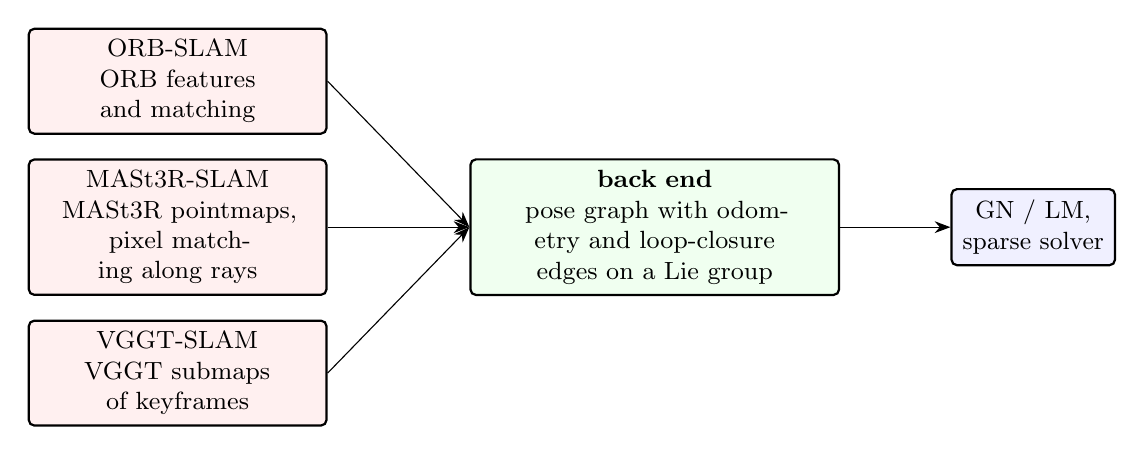
\begin{tikzpicture}[node distance=5mm]
\node[blk,text width=3.5cm,fill=red!6] (a) {ORB-SLAM\\ ORB features and matching};
\node[blk,text width=3.5cm,fill=red!6,below=3mm of a] (b) {MASt3R-SLAM\\ MASt3R pointmaps, pixel matching along rays};
\node[blk,text width=3.5cm,fill=red!6,below=3mm of b] (c) {VGGT-SLAM\\ VGGT submaps of keyframes};
\node[blk,right=18mm of b,text width=4.4cm,fill=green!6] (g) {\textbf{back end}\\ pose graph with odometry and loop-closure edges on a Lie group};
\node[blk,right=14mm of g,fill=blue!6] (s) {GN / LM,\\ sparse solver};
\draw[->] (a.east)--(g.west); \draw[->] (b.east)--(g.west); \draw[->] (c.east)--(g.west); \draw[->] (g)--(s);
\end{tikzpicture}
\caption{Same back end, different front ends (slide 40).}
\end{figure}
\begin{center}\small
\begin{tabular}{p{2.6cm}p{6.2cm}p{5.4cm}}
\toprule
 & \textbf{MASt3R-SLAM} & \textbf{VGGT-SLAM}\\\midrule
Front end & MASt3R (lecture 04) predicts pointmaps of each frame and its keyframe; pixels matched along rays & VGGT (lecture 05) reconstructs a submap of keyframes in one pass\\
Group & keyframe poses in $\Sim$ & each submap gets a homography in $\SL$ (15\,DoF)\\
Solver & Gauss--Newton, sparse Cholesky, on ray errors; loops by image retrieval & pose graph with odometry and loop-closure edges, Levenberg--Marquardt\\
Speed / camera & about 15\,FPS on one GPU; no camera model beyond a single centre & without calibration, submaps agree only up to a projective transformation\\\bottomrule
\end{tabular}
\end{center}
\begin{intuition}
Degrees of freedom of the group tell how much ambiguity the front end leaves: $\SE$ has $6$ (metric, e.g.\ stereo), $\Sim$ has $7$ (one camera: unknown scale), and $\SL$ has $15$ (an \emph{uncalibrated} reconstruction, where even angles and parallelism are not trustworthy and each submap needs a full projective correction). The back end is the same sparse least squares of Section~6.3; only the group and the residual change.
\end{intuition}
\imgph[4.2cm]{40}{MASt3R-SLAM pipeline (left) and VGGT-SLAM $\mathrm{Sim}(3)$ vs.\ $\mathrm{SL}(4)$ comparison renderings (right).}

% =====================================================================
\section{Summary \slrs{41}}
\begin{center}\footnotesize
\renewcommand{\arraystretch}{1.15}
\begin{tabular}{>{\raggedright\arraybackslash}p{2.1cm}>{\raggedright\arraybackslash}p{3.2cm}>{\raggedright\arraybackslash}p{3.1cm}>{\raggedright\arraybackslash}p{3.7cm}>{\raggedright\arraybackslash}p{3.0cm}}
\toprule
\textbf{Method} & \textbf{Estimate / variables} & \textbf{Cost} & \textbf{Loops / drift} & \textbf{Notes}\\\midrule
EKF-SLAM, MonoSLAM & current pose (13) + $N$ points, one Gaussian & $O(N^2)$ per step and memory; $\approx100$ features at 30\,Hz & no explicit loop mechanism; past poses marginalized & linearized once; may diverge\\
Factor graph / pose graph & all keyframe poses (+ points), MAP = sparse nonlinear LS & GN/LM on sparse $\bH$ (Cholesky, CG) & loop edge between non-successive poses & relinearizes; needs good initial guess\\
PTAM & tracking thread + mapping thread, BA on keyframes & BA outside the real-time loop & no large-scale loop closing & small AR workspaces\\
ORB-SLAM & ORB features; 3 threads; local BA; essential graph over $\Sim$ & local BA bounded; 21.6\,ms/image loop detection & bags of binary words; $\Sim$ corrects scale drift & relocalization $\approx78\%$ of frames\\
Continuous-time splines & control poses of a cumulative B-spline & sliding window of control poses & -- & rolling shutter: $4.7\%\to0.57\%$ error\\
Active SLAM & choose actions by utility (D-opt) & utility per candidate action & revisit vs.\ explore & active head: largest $3\sigma$ ellipsoid\\
MASt3R-SLAM / VGGT-SLAM & keyframes on $\Sim$ / submaps on $\SL$ & GN+Cholesky / LM; $\approx15$\,FPS (MASt3R) & image retrieval / pose graph loops & learned front end, same back end\\\bottomrule
\end{tabular}
\end{center}

\begin{figure}[htbp]\centering
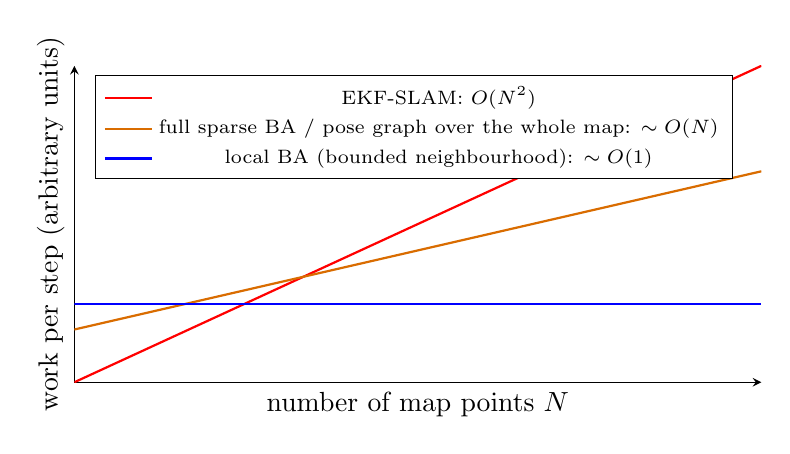
\begin{tikzpicture}
\begin{axis}[width=0.85\linewidth,height=5.6cm,xmode=log,ymode=log,xlabel={number of map points $N$},ylabel={work per step (arbitrary units)},domain=10:10000,samples=2,legend pos=north west,legend style={font=\scriptsize},axis lines=left,ticks=none]
\addplot[red,thick]{x^2/100}; \addlegendentry{EKF-SLAM: $O(N^2)$}
\addplot[orange!85!black,thick]{x}; \addlegendentry{full sparse BA / pose graph over the whole map: $\sim O(N)$}
\addplot[blue,thick]{30}; \addlegendentry{local BA (bounded neighbourhood): $\sim O(1)$}
\end{axis}
\end{tikzpicture}
\caption{Qualitative scaling of the per-step cost with the map size: the filter pays quadratically for correlations, sparse least squares roughly linearly, and keyframe-based local BA stays bounded (constants are illustrative only).}
\end{figure}

\subsection*{Key take-aways}
\begin{itemize}
\item \textbf{SLAM = joint MAP estimation} of trajectory and map from sequential frames; it is SfM with a real-time budget and loop closure.
\item \textbf{Filtering} (Bayes filter $\to$ KF $\to$ EKF-SLAM) keeps one Gaussian over the current pose and map; marginalizing past poses makes the covariance dense, so the cost is $O(N^2)$ and the map must stay tiny (about 100 features at 30\,Hz).
\item \textbf{Graph-based SLAM} keeps the keyframes: MAP on a factor graph is sparse nonlinear least squares, solved by Gauss--Newton/LM; the sparsity pattern of $\bH$ equals the graph adjacency.
\item \textbf{A modern pipeline} (ORB-SLAM) runs tracking (every frame), local mapping (local BA on the covisibility graph) and loop closing (bags of binary words, $\Sim$ pose graph to fix scale drift) in parallel.
\item \textbf{Research directions} change the front end or the problem statement: continuous time for rolling shutter, active viewpoint selection, and learned front ends (MASt3R, VGGT) on top of the same least-squares back end.
\end{itemize}

\end{document}
